%Input preamble
%Style
\documentclass[12pt]{article}
\usepackage[top=1in, bottom=1in, left=1in, right=1in]{geometry}
\parindent 22pt
\usepackage{fancyhdr}

%Packages
\usepackage{adjustbox}
\usepackage{amsmath}
\usepackage{amsfonts}
\usepackage{amssymb}
\usepackage{bm}
\usepackage[table]{xcolor}
\usepackage{tabu}
\usepackage{color,soul}
\usepackage{makecell}
\usepackage{longtable}
\usepackage{multirow}
\usepackage[normalem]{ulem}
\usepackage{etoolbox}
\usepackage{graphicx}
\usepackage{tabularx}
\usepackage{ragged2e}
\usepackage{booktabs}
\usepackage{caption}
\usepackage{fixltx2e}
\usepackage[para, flushleft]{threeparttablex}
\usepackage[capposition=top,objectset=centering]{floatrow}
\usepackage{subcaption}
\usepackage{pdfpages}
\usepackage{pdflscape}
\usepackage{natbib}
\usepackage{bibunits}
\definecolor{maroon}{HTML}{990012}
\usepackage[colorlinks=true,linkcolor=maroon,citecolor=maroon,urlcolor=maroon,anchorcolor=maroon]{hyperref}
\usepackage{marvosym}
\usepackage{makeidx}
\usepackage{tikz}
\usetikzlibrary{shapes}
\usepackage{setspace}
\usepackage{enumerate}
\usepackage{rotating}
\usepackage{tocloft}
\usepackage{epstopdf}
\usepackage[titletoc]{appendix}
\usepackage{framed}
\usepackage{comment}
\usepackage{xr}
\usepackage{titlesec}
\usepackage{footnote}
\usepackage{longtable}
\newlength{\tablewidth}
\setlength{\tablewidth}{9.3in}
\setcounter{secnumdepth}{4}

\titleformat{\paragraph}
{\normalfont\normalsize\bfseries}{\theparagraph}{1em}{}
\titlespacing*{\paragraph}
{0pt}{3.25ex plus 1ex minus .2ex}{1.5ex plus .2ex}
\makeatletter
\pretocmd\start@align
{%
  \let\everycr\CT@everycr
  \CT@start
}{}{}
\apptocmd{\endalign}{\CT@end}{}{}
\makeatother
%Watermark
\usepackage[printwatermark]{xwatermark}
\usepackage{lipsum}
\definecolor{lightgray}{RGB}{220,220,220}
%\newwatermark[allpages,color=lightgray,angle=45,scale=3,xpos=0,ypos=0]{Preliminary Draft}

%Further subsection level
\usepackage{titlesec}
\setcounter{secnumdepth}{4}
\titleformat{\paragraph}
{\normalfont\normalsize\bfseries}{\theparagraph}{1em}{}
\titlespacing*{\paragraph}
{0pt}{3.25ex plus 1ex minus .2ex}{1.5ex plus .2ex}

\setcounter{secnumdepth}{5}
\titleformat{\subparagraph}
{\normalfont\normalsize\bfseries}{\thesubparagraph}{1em}{}
\titlespacing*{\subparagraph}
{0pt}{3.25ex plus 1ex minus .2ex}{1.5ex plus .2ex}

%Functions
\DeclareMathOperator{\cov}{Cov}
\DeclareMathOperator{\corr}{Corr}
\DeclareMathOperator{\var}{Var}
\DeclareMathOperator{\plim}{plim}
\DeclareMathOperator*{\argmin}{arg\,min}
\DeclareMathOperator*{\argmax}{arg\,max}

%Math Environments
\newtheorem{theorem}{Theorem}
\newtheorem{claim}{Claim}
\newtheorem{condition}{Condition}
\renewcommand\thecondition{C--\arabic{condition}}
\newtheorem{algorithm}{Algorithm}
\newtheorem{assumption}{Assumption}
\renewcommand\theassumption{A--\arabic{assumption}}
\newtheorem{remark}{Remark}
\renewcommand\theremark{R--\arabic{remark}}
\newtheorem{definition}[theorem]{Definition}
\newtheorem{hypothesis}[theorem]{Hypothesis}
\newtheorem{property}[theorem]{Property}
\newtheorem{example}[theorem]{Example}
\newtheorem{result}[theorem]{Result}
\newenvironment{proof}{\textbf{Proof:}}{$\bullet$}

%Commands
\newcommand\independent{\protect\mathpalette{\protect\independenT}{\perp}}
\def\independenT#1#2{\mathrel{\rlap{$#1#2$}\mkern2mu{#1#2}}}
\newcommand{\overbar}[1]{\mkern 1.5mu\overline{\mkern-1.5mu#1\mkern-1.5mu}\mkern 1.5mu}
\newcommand{\equald}{\ensuremath{\overset{d}{=}}}
\captionsetup[table]{skip=10pt}
%\makeindex

\setlength\parindent{20pt}
\setlength{\parskip}{0pt}

\newcolumntype{L}[1]{>{\raggedright\let\newline\\\arraybackslash\hspace{0pt}}m{#1}}
\newcolumntype{C}[1]{>{\centering\let\newline\\\arraybackslash\hspace{0pt}}m{#1}}
\newcolumntype{R}[1]{>{\raggedleft\let\newline\\\arraybackslash\hspace{0pt}}m{#1}}



%Logo
%\AddToShipoutPictureBG{%
%  \AtPageUpperLeft{\raisebox{-\height}{
\includegraphics[width=1.5cm]{uchicago.png}}}
%}

\newcolumntype{L}[1]{>{\raggedright\let\newline\\\arraybackslash\hspace{0pt}}m{#1}}
\newcolumntype{C}[1]{>{\centering\let\newline\\\arraybackslash\hspace{0pt}}m{#1}}
\newcolumntype{R}[1]{>{\raggedleft\let\newline\\\arraybackslash\hspace{0pt}}m{#1}}

\newcommand{\mr}{\multirow}
\newcommand{\mc}{\multicolumn}

%\newcommand{\comment}[1]{}


\externaldocument{abccaretreatmenteffects_report_main_appendix}

\begin{document}
\title{\Large \textbf{Analyzing the Short- and Long-term Effects of Early Childhood Education on Multiple Dimensions of Human Development}\thanks{This research was supported in part by the American Bar Foundation; the Pritzker Children's Initiative, the
Buffett Early Childhood Fund, NIH grants NICHD R37HD065072, NICHD R01HD54702, and NIA R24AG048081, an
anonymous funder, Successful Pathways from School to Work, an initiative of the University of Chicago's Committee
on Education funded by the Hymen Milgrom Supporting Organization, and the Human Capital and Economic
Opportunity Global Working Group, an initiative of the Center for the Economics of Human Development, affiliated with
the Becker Friedman Institute for Research in Economics, and funded by the Institute for New Economic Thinking. The
views expressed in this paper are solely those of the authors and do not necessarily represent those of the funders or
the official views of the National Institutes of Health. For helpful comments, we thank St\'{e}phane Bonhomme, Steven Durlauf, and Azeem Shaikh. For information on the implementation of the Carolina Abecedarian Project and assistance in data acquisition, we thank Peg Burchinal, Carrie Bynum, Frances Campbell, and Elizabeth Gunn. For information on childcare in North Carolina, we thank Richard Clifford and Sue Russell. For very useful comments, we thank Matthew Tauzer. Lastly, we thank Sylvi Kuperman for sharing detailed and careful descriptions of the Carolina Abecedarian Project.}}

\author{
Jorge Luis Garc\'{i}a\\
The University of Chicago \and
James J. Heckman \\
American Bar Foundation \\
The University of Chicago \and
Andr\'{e}s Hojman\\
The University of Chicago \and
Yu Kyung Koh \\ 
The University of Chicago \and
Joshua Shea \\
The University of Chicago \and
Anna Ziff \\ 
The University of Chicago}
\date{First Draft: January 5, 2016\\ This Draft: \today}
\maketitle

\singlespacing
%\pagebreak
\tableofcontents
\listoffigures
\listoftables
%\pagebreak
\doublespacing

\section{Introduction}

\noindent There is a growing interest in early childhood education as a means for promoting social mobility.\footnote{\citet{Bajaj_Labaton_2009_ObamaRiskAssets,White_House_2014_Econ_of_EC_Investments,White_House_2014_Fact_Sheet_Press}.} Overall state-spending on such programs increased by 12 percent in 2015. The proposed federal budget for 2017 includes a \$300 million increase in spending on early childhood education.\footnote{\citep{US-Gov_2016_Budget,Parker-etal_2016_50-State-Review,Smith_2016_Early-Learning-Budget}.}\\

\noindent Despite the growing attention on early childhood education in public policy, comprehensive and methodologically rigorous evidence on its economic benefits is still scarce. Many recent studies: (i) focus on a limited set of outcomes that fail to capture a comprehensive array of program effects;\footnote{An extreme example is the evaluation of preschool programs using an age-eligibility cutoff. A battery of studies compare children who were just eligible and just ineligible for preschool. They therefore only assess the gains of an additional, earlier year of preschool. This does not represent a comprehensive evaluation approach; it evaluates a specific set of children for a very narrow set of tests and within a time horizon of a single year of treatment. Examples of these studies include: \citet{Gormley_Gayer_2005_JHR,Gormley_Gayer_etal_2005_DP,Weiland_2013_CD_Impacts-of-Pre-K}.} (ii) are based on data follow-ups that are short-term in nature; (iii) do not correct for program attrition or for non-compliance to assigned treatment, threatening the policy relevance of their estimates;\footnote{Consider the evaluation of Head Start through its randomized controlled trial, the Head Start Impact Study \citep{Puma_Bell_etal_2010_HeadStartImpact}. Comparing children in the treatment and the control groups usually yields relatively low gains. This attenuation happens because a substantial proportion of children randomized out of the program were enrolled into preschool alternatives, some of them to other Head Start centers. Thus, a raw comparison between the treatment- and the control-group children does not inform on either the efficiency or the effectiveness of Head Start \emph{per se}. Studies providing a methodology to account for treatment substitution find that Head Start has substantial effects, although they focus on a single, short-term outcome \citep{Kline-Walters_2015_NBER-Evaluating,Feller_Grindal_etal_2016_ComparedtoWhat}.} or (iv) are based on randomized controlled trials with flawed designs.\footnote{An evaluation of the Tennessee Voluntary Prekindergarten is an example \citep{Lipsey_et_al_2013_Tennessee_Kindergrtn_PRI,Lipsey_et_al_2015_Randomized_Control_Trial_PRI}. The researchers designed a randomized controlled trial to evaluate the program. Unfortunately, they asked permission to assess the children after the randomization protocol. Thus, their main evaluation is based on information for children whose parents agreed for them to be evaluated \textit{post} randomization, inducing a potential imbalance between the children randomized into and out of the program. The evaluation does not account for that. Further, results for this evaluation represent a narrow set of short-term outcomes.}\\ 

\noindent  The case for the long-term effectiveness and the economic efficiency of early childhood education in the U.S. is largely based on evidence from the Perry Preschool Program (referred to simply as Perry). Analyses of Perry suggest that early childhood education has significant positive effects on multiple short- and long-term socio-economic outcomes, even when accounting for compromised randomization, small-sample-size inference, and multiple hypotheses testing \citep{Heckman_Moon_etal_2010_QE}. The analyses also show that early childhood education could have an annual internal rate of return that ranges from 7 to 10 percent.\footnote{That is, if one dollar were to be invested at age 4, and then reinvested annually and compounded over a lifetime, the return would accrue to 60 to 300 dollars by age 65. This accounts for both the program's cost and the social burden a government would cause by raising taxes to pay for it \citep{Heckman_Moon_etal_2010_RateofReturn}.}\\

\noindent Critics of the empirical evidence favoring the economic case for early childhood education cite a lack of an ampler evidence base. In response, we present an integrated, rigorous evaluation of two high-quality randomized controlled trials with long-term follow-ups: the Carolina Abecedarian Project (ABC) and the Carolina Approach to Responsive Education (CARE).\\ 

\noindent ABC and CARE were programs implemented in the 1970s and early 1980s. We observe long-term outcomes for their participants. The programs were separated into two phases. In the first phase, both programs assigned high-quality center-based childcare to children from ages 0 to 5. In addition, the children who were assigned center-based childcare in CARE also received home visits that aimed to foster the relationship between participating children and their parents. Furthermore, CARE incorporated a second treatment group that received home visits without center-based childcare. The second phase of treatment, from ages 5 to 8, consisted of home visits that aimed to continue promoting childhood development. In ABC, the second-phase treatment was randomly assigned independently of the first-phase randomization. In CARE, the second-phase was not randomized; children initially randomized to either of the treatment groups maintained their assignment.\\

\noindent The data available in both programs are very similar. The data consist of measures of cognitive and socio-emotional skills, educational outcomes, labor market outcomes, administrative criminal records, and a full medical examination when subjects reached their mid-30s. Data from administrative criminal records and from the full medical panel are novel to the literature evaluating early childhood education programs. These data allow us to study the effects of early-childhood education on multiple dimensions of human development.\\

\noindent We develop a methodology to assess the effectiveness of the programs accounting for two issues that are common to experiments: (i) attrition of participants during the treatment period and subsequent follow-ups and (ii) treatment substitution by the families of the control-group children.\footnote{A usual critique to programs like ABC and CARE we do not assess here is their small sample size \citep{Hanushek_Lindseth_2009_BOOKSchoolhousesCourthouses}. Asymptotic inference methods, however, are well suited to analyze samples of the size of these programs. \citet{Campbell_Conti_etal_2014_EarlyChildhoodInvestments} evaluate the effectiveness of ABC at boosting health outcomes both using small-sample-size inference and asymptotic inference, and find little sensitivity.}\\

\noindent For each data collection stage we document non-compliance to treatment and attrition. We propose a methodology to account for these cases, which are a common critique to ABC \citep{Spitz_1992_ABC-Retardation,Hu_2014_ABC-Study}.\\

\noindent We also present a thorough documentation of control-group treatment substitution. In both programs, the parents of roughly 70\% of the children randomized out of center-based childcare enrolled their children in relatively high-quality preschool alternatives.\footnote{Treatment substitution was not an issue in Perry. Informal conversations with Perry's staff indicate that there were no alternative preschools in the area in which subjects were treated during that time---Ypsilanti, Michigan during the 1960s. This issue is more pressing when evaluating recent programs. Examples include both ABC and Head Start---see \citep{Puma_Bell_etal_2010_HeadStartImpact} for a documentation of treatment substitution in the Head Start Impact Study.} We develop a methodology to account for treatment substitution and explain that there are two policy questions that we are able to ask using data from ABC and CARE. First, we can evaluate the effect of ABC and CARE given the supply of preschool alternatives available when they were implemented. Second, we can evaluate the effect of ABC and CARE relative to a fixed alternative: no preschool at all or alternative preschools. The second question can better characterize the effectiveness of each program because it compares it to a fixed alternative.\\

\noindent We summarize the effectiveness of a program when information on multiple outcomes throughout the life-cycle is available. There are two current alternatives in the literature. One is to to calculate statistics that characterize the efficiency of a social program, such as the internal rate of return or the benefit-to-cost ratio \citep{Heckman_Moon_etal_2010_RateofReturn}. The other is to block outcomes into categories---e.g., socio-emotional skills, criminal activity, health status---and adjust the inference on each of the outcomes to account for multiple hypotheses testing and to avoid ``cherry picking'' significant results \citep{Lehman_Romano_2005_AnnStat,Lehmann_Romano_2005_testing,Heckman_Moon_etal_2010_QE}. In this paper, we calculate and formalize an inference procedure for (i) the count of outcomes for which the program causes a positive treatment effect and (ii) the count of outcomes for which the program causes a \emph{significant} and positive treatment effect, considering different levels of significance.\footnote{This alternative is an application of conducting inference on a statistic that summarizes information across multiple sources---i.e., a combining function \citep{Pesarin_Salmaso_2010_PermutationTests}.}\\

\noindent The procedure we propose accounts for multiple hypothesis testing because it does not arbitrarily pick a test of outcomes to assess treatment effects. Instead, it counts the number of outcomes for which the program has a positive (or positive and significant) treatment effect out of all available outcomes. For the same reason, it does not require arbitrarily blocking sets of outcomes when adjusting the $p$-value's to account for multiple hypotheses testing, as the standard methods do.\\

\noindent ABC's and CARE's center-based childcare from ages 0 to 5 as implemented, had substantial treatment effects on a comprehensive set of measures of human development from childhood through adulthood. For females, 79\% of the outcomes we study have a \textit{positive} average treatment effect; 37\% of the outcomes we study have a \textit{positive and significant} average treatment effect, at the 10\% level. For males, the analogous figures are 68\% and 41\%. We formalize a procedure to provide standard errors for these counts and find that they have tight confidence intervals.\footnote{These are our preferred results and account for program attrition.}\\

\noindent \textbf{[JJH: what kind of hypothesis is this?]} \\ 
\noindent \textbf{[JLG: the hypotheses are now clarified according to the last discussion we had. For the counts of positive treatment effects, the null hypothesis is for the percentage of positive treatment effects to be $\leq 50$. For the counts of positive and significant treatment effects (at the 10 \% level), the null hypotheses is for the percentage of positive and significant treatment effects to be $\leq 10$).]}\\

\noindent The effects are even stronger when accounting for treatment substitution by the families of the children who were randomized out of the main treatment  the programs offered. These effects better inform policy because they evaluate the effectiveness of the programs with respect to a well-defined counterfactual, and not as implemented.\\ 

\noindent To illustrate how accounting for treatment substitution strengthens the effects, consider one outcome for females and one outcome for males: high-school graduation and labor income at age 30, respectively. For high-school graduation rate of females, the average treatment effect when not accounting for treatment substitution amounts to an increase of 22 percentage points ($p$-value = .039); the increase amounts to 35 percentage points when accounting for treatment substitution ($p$-value = .020). For labor income for males, the average treatment effect of the programs is \$6,055 ($p$-value = .098) when not accounting for treatment substitution and \$11,310 ($p$-value = .039) when accounting for treatment substitution.\footnote{We measure labor income in 2014 USD.} This pattern sustains for a vast majority of the outcomes we consider.\\

\noindent We also test various hypotheses to assess the effectiveness of the second phase of randomization. The effectiveness of the first phase of treatment is much stronger compared to that of the second. ABC and CARE were much more effective when intervening before age 5, rather than between 5 and 8.\\

\noindent This paper extends the work of \citet{Campbell_Conti_etal_2014_EarlyChildhoodInvestments}, who analyze the effectiveness of ABC at improving long-term health outcomes. We extend the analysis by (i) assessing a multiple measures of human development; (ii) accounting for treatment substitution; and (iii) providing an alternative to test multiple hypotheses.\footnote{\cite{Campbell_Pungello_etal_2012_DP} also precede our work. The authors estimate treatment effects on adulthood outcomes in ABC. Unlike our approach, the authors do not assess outcomes such as health status, criminal behavior, and non-cognitive skills.} Furthermore, we complement the analysis by studying ABC together with CARE. The methodology and results we present underpin our companion paper, \citet{Elango_et_al_2015_ABC_unpublished}. In our companion paper, we use the treatment effects in this paper to calculate the internal rate of return and the benefit-to-cost ratio of ABC.\\

\noindent The rest of the paper proceeds as follows. Section~\ref{section:background} provides an overview of each program. It includes a description of the eligibility criteria and the populations served, a characterization of the randomization protocol and of treatment substitution, and a comprehensive summary of the treatment. Section~\ref{section:methodology} formalizes our methodology by discussing how we correct for compromised randomization and treatment substitution, and  by explaining how we test for treatment effects across multiple outcomes. Section~\ref{section:results} presents our main results and Section~\ref{section:conclusion} offers some final comments. An extensive appendix presents a much more thorough description of the program and data relative to what we present in the main text. It also discusses various alternative methodologies to evaluate the programs accounting for treatment substitution, and documents the results we present to a further extent.

\section{Background} \label{section:background}
\subsection{Overview}

\noindent The Carolina Abecedarian Project (ABC) and the Carolina Approach to Responsive Education (CARE) programs were designed and implemented by researchers at the Frank Porter Graham Center (FPGC) of the University of North Carolina in Chapel Hill. The programs targeted disadvantaged children from the semi-rural communities in the surrounding area.\\

\noindent The design and implementation of both programs was very similar. Both studies had a small sample size. ABC recruited 122 children over four cohorts, while CARE recruited 67 children over two cohorts. ABC had two phases, the first of which lasted from birth until the age of 5. In this phase, children were randomly assigned to either treatment or control groups. The treatment group received: (i) center-based childcare; (ii) breakfast, lunch, an afternoon snack, iron-fortified formula for the first 15 months of life, and a monthly supply of diapers; and (iii) medical care from licensed nurses who were supervised by a pediatrician, frequent health check-ups, and hospital referrals when serious medical treatment was needed. In contrast, the control group only received formula and diapers. In the second phase of treatment, at the age of 5, the 95 children still in the study were randomly assigned again to treatment or control groups, independently of their status in the prior randomization. This treatment consisted of home visits targeting both children and parents and lasted until age 8.\\ 

\noindent  CARE also had two treatment phases, though children were randomized only once. While the two programs had essentially identical second phases, the first phase of CARE differed significantly from the first phase of ABC by including a family education component. This component was designed to study the effects of improving the home environment on child development.\footnote{\citet{Wasik_Ramey_etal_1990_CD}.} The first treatment phase of CARE lasted from birth until the age of 5. Children were randomly assigned to one of three experimental groups: control (23 children), family education (25 children), and both family education and center-based childcare (17 children). As in ABC, the control group received diapers and complementary nutrition from birth to 15 months. The family education group received home visits that aimed to help parents solve common problems related to childrearing. Both treatment groups received the second phase of treatment from ages 5 to 8.\\

\noindent In both programs, from birth until the age of 8, data was collected annually on cognitive and socio-emotional skills, home environment, family structure, and family economic characteristics. After age 8, the collection of data was less frequent. Information on cognitive and socio-emotional skills, education, and family economic characteristics was collected at ages 12, 15, 21, and 30.\footnote{At age 30, information on cognitive skills is unavailable for both ABC and CARE.} In addition, we have two sources of data that are novel to the literature evaluating early childhood education programs: long-term measures of socio-emotional skills and administrative criminal records and a full medical panel at age 34. These rich sources of data allow us to study the long-term effects of the programs on multiple aspects of human development.

\subsection{Eligibility Criteria and Populations Served} \label{section:eligibility}

\noindent ABC recruited four cohorts of children born between 1972 and 1977. CARE recruited two cohorts of children, one born in 1978 and one in 1979. The recruitment processes in each study were identical. Potential families were referred to researchers by local social service agencies and hospitals at the beginning of the mother's last trimester of pregnancy. Eligibility was determined by a score of 11 or above in a High-risk Index (HRI).\footnote{See Appendix~\ref{appendix:background} for details on the construction of the HRI. Examples of variables in the HRI are maternal education and father's stability at work.} Table~\ref{tab:baseline} compares the children in ABC and CARE. Overall, children in CARE were relatively less disadvantaged; their mothers were older, more educated, and had higher IQ.

\begin{table}[H]
\captionsetup{singlelinecheck=false,justification=centering}
\caption{Baseline Characteristics Comparison between ABC and CARE \label{tab:baseline}}

  \begin{threeparttable}
  \begin{tabular}{cccccccc} \toprule

     &  & \scriptsize{ABC} & \scriptsize{CARE} & \scriptsize{ABC} & \scriptsize{CARE} & \mc{2}{c}{\scriptsize{$p$-value}} \\  

    \scriptsize{Variable} & \scriptsize{Age} & \scriptsize{Obs} & \scriptsize{Obs} & \scriptsize{Mean} & \scriptsize{Mean} & \scriptsize{Single $H_0$} & \scriptsize{Multiple $H_0$} \\ 
    \hline  

    \mc{1}{l}{\scriptsize{Male}} & \mc{1}{c}{\scriptsize{0}} & \mc{1}{c}{\scriptsize{116}} & \mc{1}{c}{\scriptsize{67}} & \mc{1}{c}{\scriptsize{0.464}} & \mc{1}{c}{\scriptsize{0.596}} & \mc{1}{c}{\scriptsize{\textbf{(0.060)}}} & \mc{1}{c}{\scriptsize{(0.110)}} \\  

    \mc{1}{l}{\scriptsize{Birth Weight}} & \mc{1}{c}{\scriptsize{0}} & \mc{1}{c}{\scriptsize{114}} & \mc{1}{c}{\scriptsize{64}} & \mc{1}{c}{\scriptsize{7.008}} & \mc{1}{c}{\scriptsize{7.139}} & \mc{1}{c}{\scriptsize{(0.625)}} & \mc{1}{c}{\scriptsize{(0.765)}} \\  

    \mc{1}{l}{\scriptsize{No. Siblings in Household}} & \mc{1}{c}{\scriptsize{0}} & \mc{1}{c}{\scriptsize{116}} & \mc{1}{c}{\scriptsize{67}} & \mc{1}{c}{\scriptsize{0.632}} & \mc{1}{c}{\scriptsize{0.684}} & \mc{1}{c}{\scriptsize{(0.810)}} & \mc{1}{c}{\scriptsize{(0.890)}} \\  

    \mc{1}{l}{\scriptsize{Birth Year}} & \mc{1}{c}{\scriptsize{0}} & \mc{1}{c}{\scriptsize{116}} & \mc{1}{c}{\scriptsize{67}} & \mc{1}{c}{\scriptsize{1974}} & \mc{1}{c}{\scriptsize{1979}} & \mc{1}{c}{\scriptsize{\textbf{(0.000)}}} & \mc{1}{c}{\scriptsize{\textbf{(0.000)}}} \\ 
    \midrule

    \mc{1}{l}{\scriptsize{Mother's Education}} & \mc{1}{c}{\scriptsize{0}} & \mc{1}{c}{\scriptsize{116}} & \mc{1}{c}{\scriptsize{67}} & \mc{1}{c}{\scriptsize{10.188}} & \mc{1}{c}{\scriptsize{10.868}} & \mc{1}{c}{\scriptsize{\textbf{(0.010)}}} & \mc{1}{c}{\scriptsize{\textbf{(0.025)}}} \\  

    \mc{1}{l}{\scriptsize{Mother's Age}} & \mc{1}{c}{\scriptsize{0}} & \mc{1}{c}{\scriptsize{116}} & \mc{1}{c}{\scriptsize{67}} & \mc{1}{c}{\scriptsize{19.828}} & \mc{1}{c}{\scriptsize{21.141}} & \mc{1}{c}{\scriptsize{\textbf{(0.060)}}} & \mc{1}{c}{\scriptsize{\textbf{(0.100)}}} \\  

    \mc{1}{l}{\scriptsize{Mother's IQ}} & \mc{1}{c}{\scriptsize{0}} & \mc{1}{c}{\scriptsize{116}} & \mc{1}{c}{\scriptsize{67}} & \mc{1}{c}{\scriptsize{84.407}} & \mc{1}{c}{\scriptsize{87.164}} & \mc{1}{c}{\scriptsize{\textbf{(0.070)}}} & \mc{1}{c}{\scriptsize{(0.130)}} \\  

    \mc{1}{l}{\scriptsize{Father at Home}} & \mc{1}{c}{\scriptsize{0}} & \mc{1}{c}{\scriptsize{116}} & \mc{1}{c}{\scriptsize{67}} & \mc{1}{c}{\scriptsize{0.283}} & \mc{1}{c}{\scriptsize{0.209}} & \mc{1}{c}{\scriptsize{(0.270)}} & \mc{1}{c}{\scriptsize{(0.380)}} \\  

  \bottomrule
  \end{tabular}
    \begin{tablenotes}
    \scriptsize
    \item 
    Note: This table compares baseline, observed characteristics between ABC and CARE. 
    For each characteristic, we present the $p$-value from a single hypothesis test.
    We also present the $p$-values from multiple testing, where we collectively test the
    baseline characteristics within the blocks separated by the horizontal line.
    Both $p$-values are two-sided and non-parametric. We construct them 
    based on 1,000 re-draws of the full sample. The estimates we display are the means of 
    the empirical bootstrap distribution. 
    
    \end{tablenotes}
  \end{threeparttable}

\end{table}

\noindent Though neither ABC nor CARE used race as an eligibility factor, $98\%$ and $90\%$ of their participants were African-American, respectively. On average, in ABC, mothers were 19.9 years old when the target child was born, whereas in CARE mothers were on average 21 years old. In both treatments, approximately half of all mothers were 19 years old or younger. Further, the average IQ for all mothers was 84 in ABC and 87 in CARE---approximately one standard deviation below the national mean. Only $25\%$ of the ABC children lived with both biological parents, and more than $50\%$ lived with extended families in multi-generational households ($61\%$ of treated children and $56\%$ of control children).\\

\begin{figure}[H]
\caption{Family Environment Baseline Characteristics, ABC and CARE}  \label{figure:baselineabccare}
    \centering
\begin{subfigure}{.5\textwidth}
  \centering
  \subcaption{Average Maternal Age}
  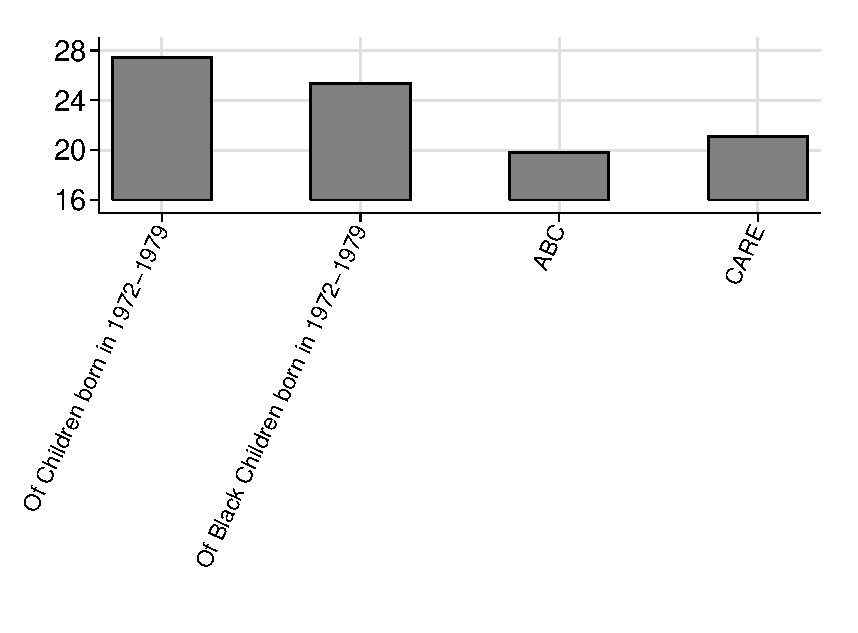
\includegraphics[height=2.3in]{output/abccarepsid_m_age0pool.eps}
\end{subfigure}%
\begin{subfigure}{.5\textwidth}
  \centering
  \subcaption{Average Maternal Years of Education} 
  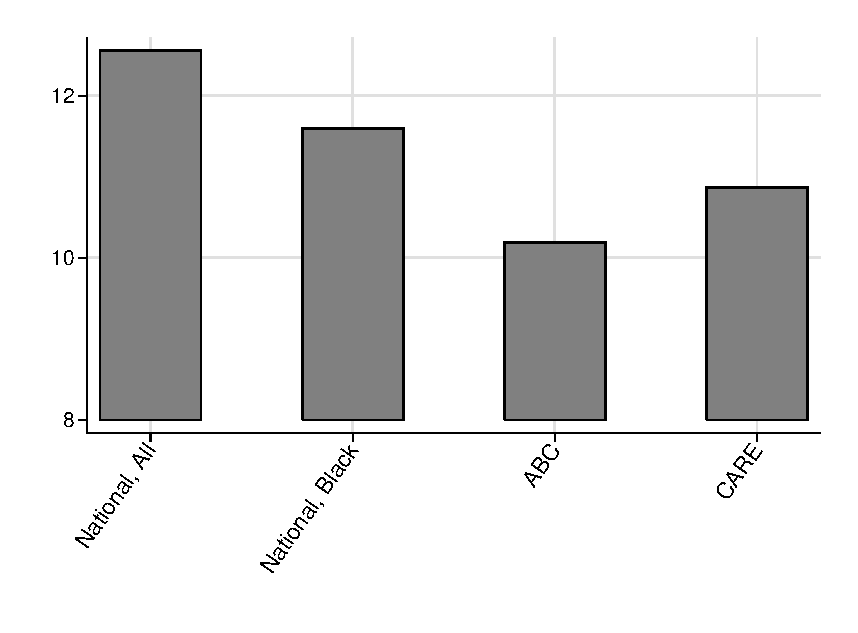
\includegraphics[height=2.3in]{output/abccarepsid_m_edu0pool.eps}
\end{subfigure}

\begin{subfigure}{.5\textwidth}
  \centering
  \subcaption{Proportion of Households with Father at Home}
  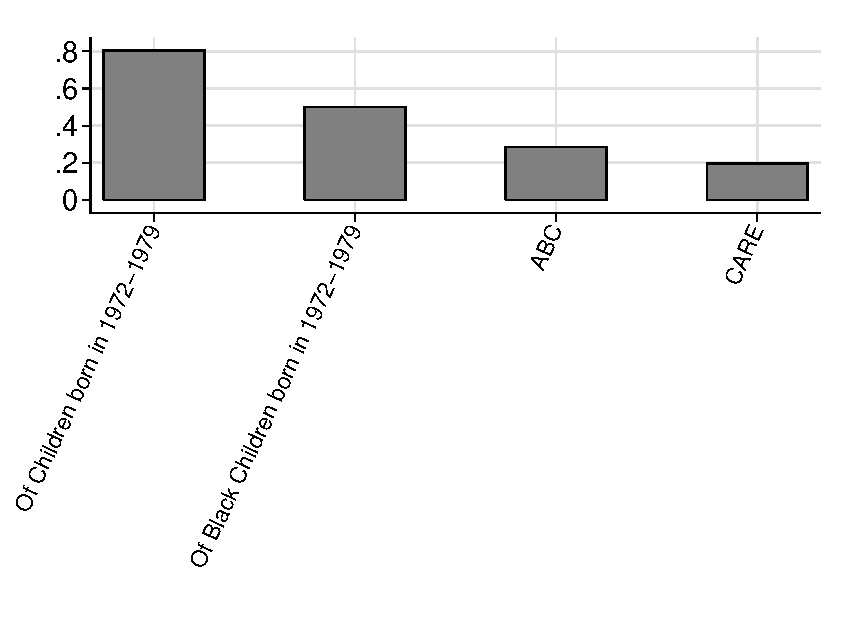
\includegraphics[height=2.3in]{output/abccarepsid_f_home0pool.eps}
\end{subfigure}%
\floatfoot{
\footnotesize
\noindent  Note: These panels plot mother's age, mother's education, and an indicator of father at home. In each panel, the first bar shows the national-level for a cohort born in the same years as the ABC and CARE individuals (1972-1979), obtained from the Panel Study of Income Dynamics (PSID). The second bar uses this same information restricted to black individuals. The third and fourth bars plot the same variables for ABC and CARE, pooling the treatment and control groups.
}
\end{figure}

\noindent To better characterize the socio-economic status of the families participating in ABC and CARE, we construct two comparison groups using the Panel Study of Income Dynamics (PSID), a nationally representative cohort of children born in the same years as the ABC and CARE participants (1972-1979), and a similar cohort restricted to black children. We show a comparison in Figure~\ref{figure:baselineabccare}. Compared to both nationally representative groups, ABC children were were born to younger, less educated mothers, most of whom were raising their children without the support of a father. The CARE participants were similarly disadvantaged compared to nationally representative groups with respect to these basic household demographic characteristics.\\

\subsection{Randomization Protocol and Compromises} \label{section:randomization}

\subsubsection{ABC}

\noindent Both the first and second phases of randomization were conducted at the family level, so pairs of siblings and twins were jointly randomized to either treatment or control groups.\footnote{Sibling pairs occurred when the two siblings were close enough in age such that both of them were eligible for the program.} Although we know that pairing was based on HRI, maternal IQ, maternal education, maternal age, and gender, we do not know the original pairs. The study collected an initial sample of 120 families. Twenty-two children did not complete the first-phase of treatment as initially assigned by the randomization (see Table~\ref{table:abccompromises}). We characterize each of the cases next and explain how to account for them in Section~\ref{section:methodology}.\footnote{In Appendix~\ref{appendix:controls}, we compare the observed, baseline characteristics of the children in Table~\ref{table:abccompromises} to the observed, baseline characteristics of the children who complied to the initial treatment assignment. We find little evidence of differences.}\\

\noindent Of these cases, there were four children assigned to treatment who left the study before any data on them was collected. The program staff did not assign them an identifier, and we classify them as Cases A, B, C, and D. In our main methodology, we assume that they are missing at random. Exercises assuming that these children had outcomes identical to the child with the lowest outcome in the treatment group suggest that, even in this extreme scenario, there is little sensitivity (see Appendix~\ref{appendix:assessingcc}).\\

\noindent Second, four children died before age 5---two of them initially assigned to treatment and two of them initially assigned to control (identifiers ``.x'', 914, 74, and 99). For all of them, we observe baseline characteristics and any other data collected before their death. For methodological purposes, they represent cases of program attrition when we do not observe their outcomes.\\

\noindent Third, three children in the treatment group did not comply to treatment status (identifiers 900, 912, 922). They are different from Cases A, B, C, and D because we observe data collected for them from birth to age 8. Afterward, the program staff chose not to follow them anymore.\footnote{Informal conversations with the program's staff do not indicate a clear reason for this.} Therefore, these children remain in treatment sample until age 8 or before. After, they represent cases of program attrition, given that we do not observe them anymore. In Appendix~\ref{appendix:assessingcc} we find little sensitivity to adjusting for non-compliance of these children in the results we show for age 8 or before.\\

\begin{sidewaystable}[H] 
\begin{threeparttable}
\caption{Randomization Compromises, ABC}
\label{table:abccompromises}
\centering
\footnotesize
\begin{tabular}{ccccc} \toprule
Child ID & Initial Assignment & Compromise Description & Data Availability & Methodology Assumption \\ \\ \midrule
Case A & Treatment & Left the study & None & Missing at random \\
Case B & Treatment & Left the study & None & Missing at random \\
Case C & Treatment & Left the study & None & Missing at random \\
Case D & Treatment & Left the study & None & Missing at random \\ \midrule
.x    & Control  & Died (age 0), heart disease & Baseline; before dead & Attrition after death \\
914 & Control  & Died (age 0), heart disease & Baseline; before dead & Attrition after death \\
74 & Treatment & Died (age 0), SIDS & Baseline; before dead & Attrition after death \\
99 & Treatment  & Died (age 4), pedestrian accident & Baseline; before dead & Attrition after death \\ \midrule
900 & Treatment  & Non-compliance  & Baseline; before age 8 & Attrition after age 8  \\
912 & Treatment  & Non-compliance  & Baseline; before age 8 & Attrition after age 8  \\
922 & Treatment  & Non-compliance  & Baseline; before age 8 & Attrition after age 8  \\ \midrule
78  & Control        & Crossover from control to treatment & Baseline; before age 8 & Attrition after age 8  \\ \midrule
85 & Treatment   & 3 months of treatment &  Baseline; after age 2 & Same as treatment group  \\  
103 & Treatment &10 months of treatment &  Baseline; after age 2 & Same as treatment group  \\
108 & Treatment & 6 months of treatment &  Baseline; after age 2 & Same as treatment group  \\ 
123 & Treatment & 9 months of treatment &  Baseline; after age 2 & Same as treatment group  \\  \midrule
906 & Control  & Left study at 54 months & Baseline; before 54 months & Attrition after 54 months \\ \midrule
95   & Treatment       & Developmentally delayed at 6 months & No data after diagnosis & Dropped (non-eligible) \\ 
124 & Treatment       & Developmentally delayed at 36 months & No data after diagnosis & Dropped (non-eligible) \\ \midrule
 82 & Control       & Crossover from control to treatment & Baseline, before age 8 & Dropped (non-eligible)  \\ 
 119 & Control       & Crossover from control to treatment & Baseline, before age 8 & Dropped (non-eligible)  \\ \bottomrule
\end{tabular}
\begin{tablenotes}
\item Note: This table describes the various randomization compromises in ABC. For each child, we display: the ID assigned by the program staff, the nature of the compromise, the data available, and the methodological assumption when accounting for non-compliance and program attrition. 
\end{tablenotes}
\end{threeparttable}
\end{sidewaystable}

\noindent Fourth, one child initially assigned to control was enrolled into treatment (identifier 78). Her mother wanted to work and the program staff decided to admit her child in center-based care.\footnote{Correspondence with the program officers stating this permission is available under request from the authors.} Both in terms of data collection and in terms of methodological purposes, this child is analogous to the children in the third case.\footnote{The sensitivity analysis finding little evidence when adjusting for non-compliance includes this case.}\\

\noindent Fifth, four children in the treatment group did not complete treatment in its entirety (identifiers 85, 103, 108, and 123). They were treated for 3, 10, 6, and 9 months, respectively. Except for follow-ups during childhood, which our main results do not use, we observe most of the data for these children. We avoid taking a stance on how beneficial the program was at each age, because we do not have a way to document this. Therefore, we assume that they were treated as other child in the treatment group.\footnote{If anything, this downward biases the effects of the program we estimate.} \\

\noindent Sixth, the family of one child in the control group moved at age 54 months (identifier 906). We observe any data collection before the family moved, so we consider the child as part of the control group in any estimation before this event. Afterwards, we do not observe any data on the child, so we consider her a case of program attrition.\\

\noindent Seventh, two children initially assigned to treatment status were diagnosed as developmentally delayed after six and thirty-six months of treatment (identifiers 95 and 124, respectively). No data for them are available after the diagnosis. We drop them from the sample because they were not eligible to be part of the program, to begin with, as we explain in Section~\ref{section:eligibility}.\\

\noindent Finally, two children initially assigned to the control group were admitted into treatment (identifiers 82 and 119). Local authorities requested this because the children were considered highly at risk. Data on them is available from birth and up to age 8 and we treat them as the children in the third and fourth cases. They crossed over from the control group to the treatment group, although the reasons were different.\\

\noindent Analysis of each of these cases leads to the following conclusions. For four children, we do not have data to methodologically assess them as cases of program attrition, though sensitivity analyses suggest that the treatment effects of the program persist after assigning them the same outcome as the children who did worst in the treatment group. For the children who did not comply to treatment, adjusting our estimates for non-compliance when data is available makes little difference. The remaining 14 children who did not complete treatment as initially assigned represent various cases of program attrition, for which we propose a correction methodology in Section~\ref{section:methodology}.\\

\noindent To increase the number of children in the sample, the program officers recruited additional children who were added to the program before children were six months old. Our calculations indicate that there were eight replacements. We cannot distinguish in the data the children who were initially randomized from the substitute children and there is no documentation on how these children were recruited.\footnote{Three replacements are reported in \citet{Ramey_Campbell_1979_SR}. Three are documented in correspondence with the program officers, which is available from the authors of the present document upon request. The other two replacements are implied by the number of children who participated of the randomization protocol in each cohort.} After the various compromises, the sample consisted of 111 children: 53 in the treat group and 58 in the control group. The observed characteristics for each child indicate that they were eligible for the program; all children in the sample have an HRI of 11 or above. \\

\noindent Prior to the second phase of randomization, 3 children in the first-phase control group and 3 children in the first-phase treatment group could not be located for follow-up. One child in the control group and 8 children in the treatment group of the first phase did not participate in the second phase but later agreed to participate in the data collections during adulthood. This yielded a sample of 96 children in the second phase: 49 in treatment and 47 in control. After the second-phase randomization, three children in the treatment group chose not to participate in the program, while all children in the control group adhered to their randomization status. Figure~\ref{fig:abc-flow} in Appendix~\ref{appendix:background} illustrates ABC's randomization protocol and the flow of participants throughout the data follow-ups.\\

\subsubsection{CARE}

\noindent The randomization protocol in CARE had no major compromises.\footnote{\citet{Wasik_Ramey_etal_1990_CD,Burchinal_Campbell_etal_1997_CD}.} Of the 65 initial families, 23 were randomized to control, 25 to the family education treatment group, and 17 to the family education and center-based childcare treatment group. Two families in the family education treatment group had twins who were jointly randomized, as in ABC. We document four cases of program attrition (see Table~\ref{table:care_compromises}).\footnote{In Appendix~\ref{appendix:controls}, we compare the observed, baseline characteristics of the children in Table~\ref{table:care_compromises} to the observed, baseline characteristics of the children who complied to the initial treatment assignment. We find little evidence of differences.} For methodological purposes, we consider these children analogous to their corresponding cases in ABC. We do not present exercises to evaluate the sensitivity to non-compliance because there was none in CARE. Figure~\ref{fig:care-flow} in Appendix~\ref{appendix:background} illustrates CARE's randomization protocol and the flow of participants throughout the data follow-ups.\\

\begin{sidewaystable}[H] 
\begin{threeparttable}
\caption{Randomization Compromises, CARE}
\label{table:care_compromises}
\centering
\footnotesize
\begin{tabular}{ccccc} \toprule
Child ID & Initial Assignment & Compromise Description & Data Availability & Methodology Assumption \\ \\ \midrule
310 & Family education & Died (age 0), unknown causes & Baseline & Attrition after dead \\
301 & Center-based Childcare and Family Education  & Left study at age 5  & Baseline; before age 5 & Attrition after age 5 \\
910 & Control & Move at 11 months old & Baseline; before 11 months & Attrition after 11 months \\
142 & Center-based Childcare and Family Education & Move at 5 months old & Baseline; before 5 months & Attrition after 5 months \\
150 & Center-based Childcare and Family Education & Move at age 5 & Baseline; before age 5 & Attrition after 5 \\ \bottomrule
\end{tabular}
\begin{tablenotes}
\item Note: This table describes the various randomization compromises in CARE. For each child, we display: the ID assigned by the program staff, the nature of the compromise, the data available, and the methodological assumption when accounting for non-compliance and program attrition. 
\end{tablenotes}
\end{threeparttable}
\end{sidewaystable}

\subsection{Program Description and Content}

\noindent The ABC and CARE programs shared many objectives and program characteristics, as summarized in Table~\ref{tab:programcomparison}.\\

\begin{table}[H]
\begin{center}
\begin{threeparttable}
\caption{ABC and CARE, Programs Comparison} \label{tab:programcomparison}
\scriptsize
\scalebox{.9}{\begin{tabular}{L{4cm} L{7cm} L{5cm}}
\hline \hline
& \multicolumn{1}{c}{ABC}& \multicolumn{1}{c}{CARE}\\
\hline 
Program Overview &&\\
\hspace{.5cm} Years Implemented &1972--1982&1978--1985\\
\hspace{.5cm} Age of Entry/Exit & birth to 5 years old &\checkmark\\
\hspace{.5cm} Initial Sample &122&64\\
\hspace{.5cm} \# of Cohorts &4&2\\
\midrule
Eligibility & socio-economic disadvantage according to a multi-factor index (see Section \ref{section:eligibility})&\checkmark\\
 \midrule
Control &&\\
\hspace{.5cm} N &54&23\\
\hspace{.5cm} Compensation & Diapers from birth to age 3, unlimited formula from birth to 15 months & \checkmark \\
\hspace{.5cm} Treatment Substitution & 70\% & $\sim$ 70\%\\
\midrule
Treatment & Center-based childcare & Center-based childcare and family education\\
\hspace{.5cm} \textbf{Center-base} &&\\
\hspace{.5cm} \textbf{Childcare} &&\\
\hspace{.5cm} N &57&17\\
\hspace{.5cm} Intensity &6.5--9.75 hours a day for 50 weeks per year&\checkmark\\
\hspace{.5cm} Components & Instruction, medical care, nutrition, social services &\checkmark\\
\hspace{.5cm} Staff-to-child Ratio &1:3 during ages 0--1 &\checkmark\\
&1:4--5 during age 1--4 &\checkmark\\&1:5--6 during ages 4--5 &\checkmark\\
\hspace{.5cm} Staff Qualifications &Mixed diplomas; experienced&\checkmark\\
\hspace{.5cm} \textbf{Family Education} & Not part of the program &24\\
\hspace{.5cm} Intensity && One hour-long home visits. 2--3 per month during ages 0--3. 1--2 per month during ages 4--5\\
\hspace{.5cm} Curriculum & & Social and mental stimulation; parent-child interaction\\
\hspace{.5cm} Staff-to-child Ratio &&1:1\\
\hspace{.5cm} Staff Qualifications &&Home visitor training\\
\midrule
 School-age Treatment \\
 \hspace{.5cm} N&46&39\\
\hspace{.5cm} Intensity &Every other week& \checkmark\\
\hspace{.5cm} Components &Parent-teacher meetings& \checkmark\\
\hspace{.5cm} Curriculum & Reading and math &\checkmark\\
\hspace{.5cm} Staff-to-child Ratio &1:1&\checkmark\\
\hspace{.5cm} Staff Qualifications &Graduate degree and training in special education & \checkmark\\
\midrule
Data Availability \\
Questionnaires & Ages 0--5, 8, 12, 15, 21, 30--34 & Ages 0--5, 8, 12, 21, 30--34 \\
Parent Interview & Ages 0--5, 8, 12, 15, 21& Ages 0--5, 9, 12 \\  
Health Follow-up & Ages 30--34&\checkmark\\
\hline \hline
\end{tabular}}
\footnotesize
\begin{tablenotes}
\item Note: This table compares the main elements of ABC and CARE, summarized within this section.
\end{tablenotes}
\end{threeparttable}
\end{center}
\end{table}

\noindent ABC and CARE shared a main objective: to prevent ``mental retardation" and to develop school readiness for disadvantaged children, starting at birth.\footnote{Note that the clinical understanding of mental retardation was once associated with disadvantages that hindered early-life development \citep{Mental-Retardation_America_2004_BOOK_NYU}.} The different curricula implemented across programs and cohorts had the following common goals: (i) to support language and cognitive development and (ii) to develop socio-emotional competencies that were considered to enable school-readiness---e.g., task orientation, emotional self-expression, independence, sharing, and cooperation.\footnote{\citet{Sparling_1974_Synth_Edu_Infant_SPEECH,Ramey_Collier_etal_1976_CarolinaAbecedarianProject,Ramey-etal_2012-ABC}.} The curricula evolved each year according to recommendations made in studies that used the children's data.\footnote{\citet{Ramey-etal_1975_AJoMD,Finkelstein_1982_Day_Care_YC,Haskins_1985_CD}.}$^{,}$\footnote{The curricula implemented in the first phases of ABC and CARE, including Tools of Mind, shared an emphasis on self regulation---e.g., goal setting and self-reflection---and opportunities for language development. Language development, including phonics and reading skills, is also an important element in other widely implemented curricula such as Opening the World of Learning.}$^{,}$\footnote{Two other renowned early childhood education programs are worth comparing to ABC and CARE. The Infant Health and Development Project (IHDP) was based on the first phase of CARE. IHDP had a single treatment group, which was very similar to the center-based childcare and family education treatment group of CARE. The curricula implemented both at home and at center-based childcare were very similar. The main difference is that the first phase of CARE lasted 5 years, while IHDP lasted 3 years and did not have a second phase. Both ABC and CARE were notably different from the Nurse Family Partnership (NFP) program. NFP had fewer visits and began in the pre-natal period. Mothers received monthly visits during pregnancy and one visit every two months from when the child was born until the age of 2. The visitors were nurses and they tried to help women build relationships with friends and family to create a support network for their children. A common element of the three programs is that the visitors helped parents use community resources when solving their everyday problems.}\\

\noindent Both treatment groups in CARE incorporated home visits, which aimed to help parents resolve everyday problems that could adversely affect relationships with their children, as well as to improve the general skills associated with parenting. Generally, the home visits were weekly and one hour long. Between birth and the age of 3, participants in both treatment groups received, on average, 2.5 and 2.7 visits a month, respectively. At ages 4 and 5, the average frequency decreased to 1.4 and 1.1 visits per month.\\ 

\noindent The first phases of ABC and CARE were conducted in conjunction with a longitudinal medical research study on infectious respiratory diseases in group environments.\footnote{\citet{Henderson-et-al_1982_NEJoM}.} This study meant that children had comprehensive medical care in the same center in which they received center-based childcare. The children who attended the center received daily screenings to detect any signs of illness. This included all the children in the treatment group of ABC and all the children in the center-based childcare and family education group of CARE. The first cohort of the control group of ABC also received frequent medical check-ups during the first year of the first-phase of the program.\\

\noindent The children assigned to treatment in the first phase of ABC also received primary pediatric care by a family nurse practitioner and a licensed practical nurse, who were supervised by a pediatrician on continuous duty at the childcare center. This care consisted of wellness check-ups, immunizations, parental counseling, and initial assessments of illnesses. Like the other treatment components, pediatric care was free of charge. Unfortunately, there is no documentation or corresponding evidence for whether this aspect of treatment was available to the center-based childcare and family education treatment group of CARE.\\

\noindent For both ABC and CARE, children in the programs' center-based childcare were provided breakfast, lunch, and an afternoon snack, planned by a nutritionist. Children in the control groups of both programs received diapers from birth until the age of 3, and an unlimited supply of bottled formula from birth until 15 months. Neither of the control groups in both programs nor CARE's family education treatment group received any program-sponsored medical care, with the exception of the first cohort of control children in ABC, as explained above.\\

\noindent The second phase of both ABC and CARE, also referred to as school-age treatment, lasted for the first three years of elementary school and consisted of home visits by a teacher. The visits aimed to increase the children's exposure to reading and mathematics and to promote parental involvement in the learning process. These visits occurred every two weeks in the presence of the parents. During their visits, teachers discussed the children's curricula and helped parents with issues related to literacy, housing, and medical care.\\

\subsection{Treatment Substitution}

\noindent When comparing the treatment and control groups in both programs, the interpretation of this comparison depends on how the control group substituted for treatment. This behavior poses a methodological challenge when trying to construct estimates that answer policy-relevant questions. In both programs, many children without access to center-based childcare through random assignment nevertheless attended alternative preschools. In this section, we characterize the types of care received by the treatment group. We propose a methodology to answer policy-relevant questions in Section~\ref{section:methodology}.\\

\begin{figure}[H]
		\caption{Treatment Substitution, ABC} \label{fig:treatsubabc}
		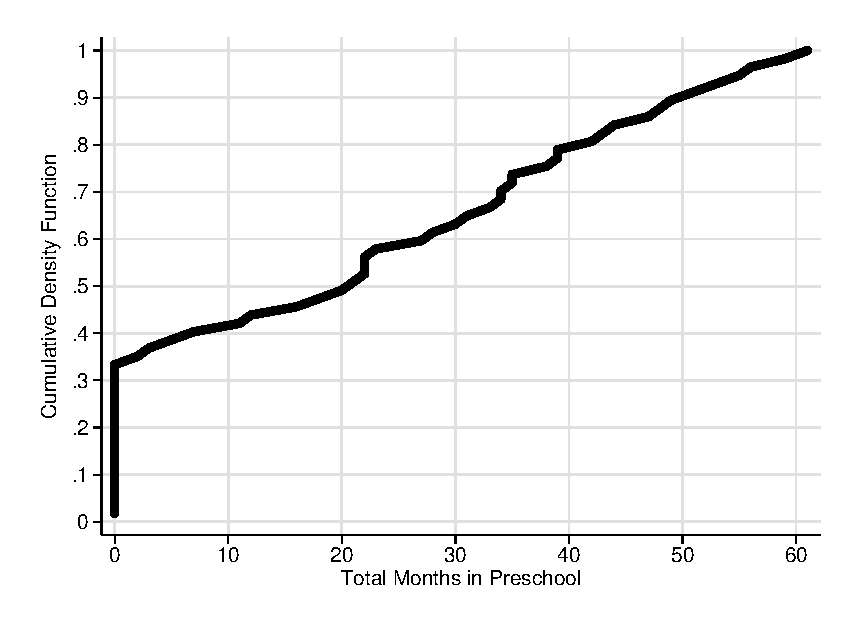
\includegraphics[width=.9\columnwidth]{output/abc_controlcontamination_months.eps}
\floatfoot{
\footnotesize
\noindent Note: This figure displays the cumulative density function of enrollment in an alternative preschool for the control group in ABC.}
\end{figure}

\noindent In ABC, $66\%$ of control-group children were enrolled in one of 11 local center-based childcare centers (see Figure~\ref{fig:treatsubabc}). Each of these centers received federal subsidies and were therefore regulated by the Federal Interagency of Daycare Requirements. Therefore, their staff members were required to be trained in early childhood education, and the centers were required to implement approved curricula designed to enhance cognitive, social, and linguistic competence in disadvantaged children.\footnote{\citet{Burchinal_etal_1989_CD_Daycare-Pre-K-Dev}.} In CARE, $74\%$ of the control group and $59\%$ of the family education group were enrolled in alternative preschools by their parents (see Figure~\ref{fig:treatsubcare}). Parents in both of these groups had as options the same set of local center-based childcare centers as the ABC children in the control group.

\begin{figure}[H]
		\caption{Treatment Substitution, CARE} \label{fig:treatsubcare}
		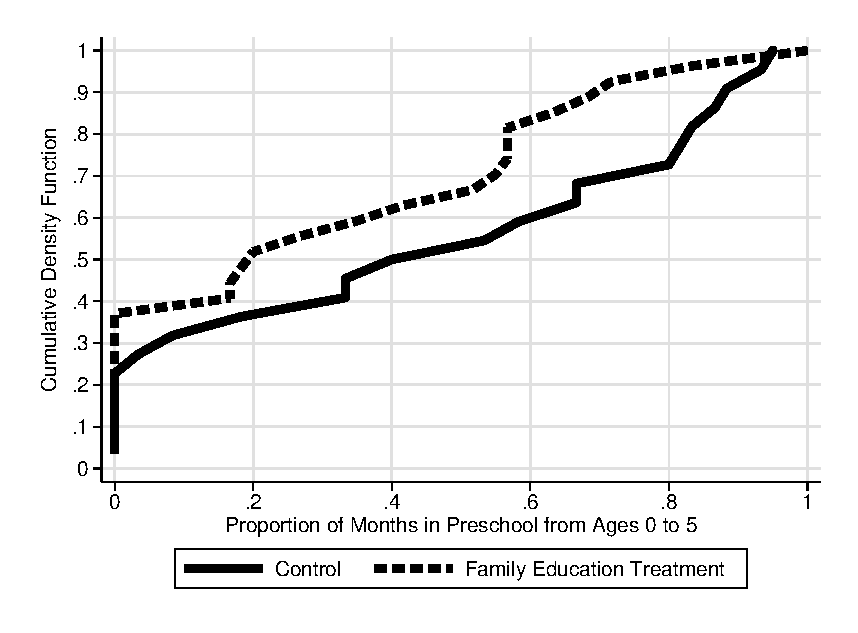
\includegraphics[width=.9\columnwidth]{output/care_controlcontamination_months.eps}
\floatfoot{
\footnotesize
\noindent Note: This figure displays the cumulative density function of enrollment in an alternative preschool for the control and family education treatment groups in CARE.}
\end{figure}

\noindent The available documentation indicates that the preschool alternatives were of high-quality. Most received federal subsidies and, therefore, were regulated by the Federal Interagency of Day Care Requirements. They were required to have trained staff who were able to implement curricula designed to enhance cognitive, social, and linguistic competence in disadvantaged children.\footnote{\citet{Burchinal_etal_1989_CD_Daycare-Pre-K-Dev}.} We document this more thoroughly in Appendix~\ref{appendix:background}.

\subsection{Data} \label{section:data}

\begin{sidewaystable}
\caption{Data Availability (Part I)} \label{tab:datasumm_1}
\centering
\scriptsize
\setlength{\tabcolsep}{0.5em} % for the horizontal padding
{\renewcommand{\arraystretch}{1.8}%
\begin{tabular*}{\textwidth}{L{2cm} C{3.5cm} C{2.8cm} C{2.8cm} C{2.5cm}  C{2.5cm} C{2cm} C{2cm}} \toprule
 & &\multicolumn{2}{c}{Early Childhood} &  \multicolumn{2}{c}{Childhood and Adolescence} &  \multicolumn{2}{c}{Adulthood} \\
Category & Sub-category & ABC Age (in months) & CARE Age (in months) & ABC Age & CARE Age  & ABC Age & CARE Age  \\
\midrule
Demographics & Gender & Birth, 18, 30, 42, 54  & Birth, 18, 30, 42, 54 & - & - & - & - \\
 & Race  & Birth, 18, 30, 42, 54  & Birth, 18, 30, 42, 54 & - & - & - & - \\
 & Birth date & Birth, 18, 30, 42, 54  & Birth, 18, 30, 42, 54 & - & - & - & - \\
 \midrule
Physical Health & Growth data (e.g. height, weight) & 3, 6, 9, 12, 18, 24, 36, 48, 60 & Birth, 6, 12, 18, 24, 36, 48, 60 & - & - & - & - \\
 & Health issues & - & - & 8, 12, 15 & 8, 12 & 21, 30 & 21 \\
  & Full medical sweep & - & - & - & - & 34 & 34 \\
 \midrule
Family Environment & Family Members (e.g. marital status of parents) & Birth, 6, 18, 30, 42, 54 & Birth, 6, 18, 30, 42, 54, 60 & 6, 8, 12, 15 & 7, 8, 12 & 21, 30 & 30 \\
 & Family Economic Environment (e.g. parent occupations) & Birth, 18, 30, 42, 54 & Birth, 18, 30, 42, 54 & 6,8,12,15 & 5,7,8,12 & 21 & 30 \\
 & Family Social Status (e.g. parents' education ) & Birth, 18, 30, 42, 54 & Birth, 6, 18, 30, 42, 54, 60 & 6, 8, 12, 15 & 7, 8, 12 & - & - \\
 & Physical Health of Family Members & Birth & Birth & 8, 12, 15 & 12 & - & - \\
 & Marital Status & - & - & - & - & 21, 30 & 21,30 \\
 & Number of Children & - & - & - & - & 21, 30 & 30 \\
 \midrule
Childcare & Day-care Experience & Birth, 18, 30, 42, 54 & 6, 18, 30, 42, 54 & - & - & - & - \\
 & Parental Care & 6, 18, 30, 42, 54 & 6, 12, 18, 30, 42, 54 & - & - & - & - \\
 \midrule
Cognitive Assessments & Intelligence Levels & 3, 6, 9, 12, 15, 24, 15, 18, 24, 36, 48, 60 & 6, 12, 18, 24, 36, 48, 60 & 6, 7, 8, 12, 15 & 6, 7, 8, 12, 15 & 21 & - \\
 & Language Ability & 36, 42, 48, 54 & 30, 42, 54 & 6, 7, 8, 12 & 6, 7, 8 & - & - \\
 & Motor Development & 3, 6, 9, 12, 18, 24, 30, 42, 54 & 6, 12, 18, 24, 30, 42, 54 & 7 & 6 & - & - \\
 & Critical Thinking & 30, 36, 42, 48, 54, 60, 66, 72 & - & 6, 7, 8 & 8, 12 \\
 \bottomrule

\end{tabular*}}
\begin{tablenotes}
\scriptsize
\item Note: This table describes the major categories of variables that were measured for ABC and CARE subjects. This is not an exhaustive list of variables, nor does it include variables from auxiliary data. Each age listed indicates that one or more measures of the given variable were collected from the subject at that age. Measures are collected using standardized assessments, interviews, or questionnaires. 
\end{tablenotes}
\end{sidewaystable}

\begin{sidewaystable}
\caption{Data Availability (Part II)} \label{tab:datasumm_2}
\centering
\scriptsize
\setlength{\tabcolsep}{0.5em} % for the horizontal padding
{\renewcommand{\arraystretch}{1.8}%
\begin{tabular*}{\textwidth}{L{2cm} C{3.5cm} C{2.8cm} C{2.8cm} C{2.5cm}  C{2.5cm} C{2cm} C{2cm}} \toprule
 & &\multicolumn{2}{c}{Early Childhood} &  \multicolumn{2}{c}{Childhood and Adolescence} &  \multicolumn{2}{c}{Adulthood} \\
Category & Sub-category & ABC Age (in months) & CARE Age (in months) & ABC Age & CARE Age  & ABC Age & CARE Age  \\
\midrule
Non-Cognitive Assessments & Social Skills & 30, 36, 42, 48, 54, 60, 66, 72  & 6, 12, 18, 24 & 6, 8, 12, 15 & 8, 12 & 21, 30 & 21, 30 \\
 & Self Control & 3, 18, 30, 36, 42, 48, 54, 60, 66, 72 & 6, 12, 18, 24 & 6, 7, 8, 12, 15 & 12 & 21, 30 & - \\
 & Self-Consciousness & 30, 36, 42, 48, 54, 60, 66, 72 & - & 8, 12, 15 & 8, 12 \\
 & Work Ethic & - & - & 6, 7, 8, 12, 15 & 6, 7, 8, 9, 12 \\
 & Social Activities & - & - & 8, 12, 15 & 8, 12 & 21, 30 & 21, 30 \\
 \midrule
Academic Achievements & Standardized Tests & - & - & 6, 7, 8, 12 & 6, 8, 9, 12 & - & - \\
 & Performance in School & - & - & 12, 15, 17 & 11, 12 & - & - \\
 & Education Level & - & - & - & - & 21,30 & 21,30 \\
 \midrule
Economic Status & Living Circumstances & - & - & - & - & 21, 30 & 21, 30 \\
 & Working Condition (e.g. job title \& category) & - & - & - & - & 21, 30 & 21, 30 \\
 & Income & - & - & - & - & 21, 30 & 21, 30 \\
 \midrule
Social Conduct & Administrative Criminal Records & - & - & - & - & mid-30s & mid-30s \\
& Law Breaking & - & - & 15 & - & 21 & 21, 30 \\
 & Risk Taking (e.g. smoking, drinking) & - & - & - & - & 21, 30 & 21, 30 \\
\toprule
\end{tabular*}}
\begin{tablenotes}
\item Note: This table describes the major categories of variables that were measured for ABC and CARE subjects. This is not an exhaustive list of variables, nor does it include variables from auxiliary data. Each age listed indicates that one or more measures of the given variable were collected from the subject at that age. Measures are collected using standardized assessments, interviews, or questionnaires. 
\end{tablenotes}
\end{sidewaystable}

\noindent Table~\ref{tab:datasumm_1} and Table~\ref{tab:datasumm_2} summarize the available data. The data collection process was analogous in both programs. The treatment and control groups were followed into adulthood with relatively low attrition compared to other long-term studies. For ABC, children were followed annually through elementary school and at ages 12, 15, 21, and 30. Health and administrative crime data were collected when the children reached their mid-30s. For CARE, the exact same follow-ups are available, with the exception of the age 15 follow-up.\\

\noindent Information on developmental progress, schooling, home environment, and parental characteristics was recorded through early childcare, elementary school, and at age 21. The data include measures of the child's IQ, achievement test scores, health status, risky behavior, schooling, social interactions, socio-emotional status, and non-cognitive skills. The data also include family and household variables, such as parents' labor market participation, household income, parental IQ, parental schooling, and parental attitudes toward child-rearing. For ages 21 and 30, information on labor market outcomes, income, educational attainment, relationship histories, health statuses, household statuses, risky behavior, and criminal activity is available.\\

\noindent For ABC, information is available on 100 children in the age 30 follow-up, which we call the adult follow-up. In addition, 80 participants---40 from the control group and 40 from the treatment group---consented to the release of their criminal records. Further, 70 participants consented to the release of information regarding a full-range biomedical panel---31 from the control group and 39 from the treatment group. Examples of measures in the health data include incidence of diabetes and high blood pressure, waist-to-hip ratio, height and weight, and cholesterol levels. Similar data is available for CARE. In Appendix~\ref{appendix:randomization}, we document balance in observed, baseline characteristics across the treatment and control groups, once we drop the individuals for whom we have crime or health information. Further, the methodology we propose addresses missing information in either of these two data categories.

\section{Methodology} \label{section:methodology}

\subsection{Parameters of Interest and Policy Questions} \label{section:methodsquestions}

\noindent Random assignment does not guarantee that conventional treatment effect estimates used in the literature are able to answer policy-relevant questions. For an estimator to be useful in policy design, it should relate to a relevant parameter by clearly stating the counterfactual scenario to which the evaluated program is being compared.\\

\noindent In this section, we outline our methodology for estimating policy-relevant parameters. We start by comparing children who \textit{take up} treatment to children who do not. For the moment, we focus our exposition on estimating the effect of ABC's first phase of treatment, center-based childcare. We then clarify how to incorporate the second phase of treatment into our estimates---as well as the multiple, simultaneous treatments offered in CARE.\\

\noindent Let $D = 1$ if the child takes up center-based childcare, and $D=0$ if the child does not. Let $Y$ be an outcome of interest. We write

\begin{equation}
Y = Y_{0} + D \left( Y_{1} - Y_{0} \right) \label{eq:outcome}
\end{equation}

\noindent where $Y_{1}$ is the child's potential outcome if she takes up treatment, and $Y_{0}$ is the child's potential outcome if she does not---i.e., $Y_{1}$ is her outcome when fixed to take up treatment and $Y_{0}$ when she is fixed not to.\\

\noindent The conventional method of evaluating a program's treatment effect is to compare the expectation of $Y_{1}$ to the expectation of $Y_{0}$, which captures the average treatment effect. That is, test the following hypothesis:

\begin{equation}
H_{0}^A: \mathbb{E} \left[ Y_{1} \right]  = \mathbb{E} \left[ Y_{0} \right]. \label{eq:ho}
\end{equation}

\noindent We can extend this method to testing various other hypotheses, such as differences in higher order moments and rank.

\noindent \begin{definition} \label{assumption:pc} \normalfont (Perfect Compliance) Let $R$ indicate randomization to treatment and $D$ indicate treatment take-up. Perfect compliance occurs whenever  $R = D$.\end{definition}

\noindent Under perfect compliance, testing~\eqref{eq:ho} is equivalent to testing if the intent-to-treat (ITT) estimator is different from zero. This estimator is defined as 

\begin{equation}
\text{ITT} := \mathbb{E} \left[ Y | R = 1 \right] - \mathbb{E} \left[ Y | R = 0 \right]. \label{eq:itt}
\end{equation} 

\noindent To relate the ITT to a policy-relevant parameter note that

\begin{align}
\text{ITT} &= \mathbb{E} \left[ Y | R = 1 \right] - \mathbb{E} \left[ Y | R = 0 \right] \nonumber \\
	       &= \mathbb{E} \left[ Y_{0} + D \left( Y_{1} - Y_{0} \right)  | D = 1 \right] - \mathbb{E} \left[ Y_{0} + D \left( Y_{1} - Y_{0} \right)  | D = 0 \right] \nonumber \\
	       &= \mathbb{E} \left[ Y_{1} \right] - \mathbb{E} \left[ Y_{0} \right] \nonumber \\
	       &=: \text{Average Treatment Effect (ATE)}, 
\end{align} 

\noindent where the second equality follows from Definition~\ref{assumption:pc} and from the definition of $Y$ in \eqref{eq:outcome}. As a policy parameter, the ATE answers the following question: What is the expected effect of fixing a randomly selected individual to treatment status, relative to fixing her to control status?\\

\noindent In practice, ABC had cases of non-compliance and program attrition. Therefore, the ITT does not recover $ \mathbb{E} \left[ Y_{1} \right] - \mathbb{E} \left[ Y_{0} \right] $ and does not provide a statistic to test the hypothesis specified in \eqref{eq:ho} without further adjustment. In the study, children who did not comply with their assignment were not followed beyond age 8, at which point program treatment had ended. Since we focus on outcomes after this age, we will propose a methodology to correct for program attrition and not for imperfect compliance. Additionally, we find that outcomes before age 8 are mostly insensitive to issues of non-compliance (see Appendix~\ref{appendix:assessingcc}).\\

\subsection{Accounting for Attrition}

\noindent To account for program attrition in our estimation, we develop a correction to the ITT formula, which could be generalized to test differences in high order moments or rank. Let $A$ be an indicator of program attrition and $Y_{d} $ represent a potential outcome, where $d$ indexes program take-up. It is not necessarily the case that 

\begin{equation}
\mathbb{E} \left[ Y_{d} |  A = 1 \right]  = \mathbb{E} \left[ Y_{d} | A = 0  \right],
\end{equation}

\noindent which motivates the following assumption. 

\begin{assumption} \normalfont \label{assumption:balance} (Conditional Independence in Program Attrition) The expectation of potential outcome $Y_{d}$ is independent of $A$ after conditioning on observed characteristics, $X$: 

\begin{equation}
\mathbb{E} \left[ Y_{d} | A = a, X \right] = \mathbb{E} \left[ Y_{d} | X \right].
\end{equation}

\end{assumption}

\noindent Under Assumption~\ref{assumption:balance}, we can correct for program attrition in our estimation of the ITT by using inverse probability weighting (IPW). Once this correction is applied, the ITT provides an estimate of the ATE. In other words, we can weight observations in the data to achieve balance in observed characteristics between children for whom data was collected and not collected. Assumption~\ref{assumption:balance} states that once $X$ is balanced, conditioning on program attrition has no bearing on the potential distributions of interest. Therefore, these distributions are identifiable. Once we account for program attrition, the ITT represents the average treatment effect of ABC with respect to the control group. For clarity, we omit $A$ henceforth, although in our empirical application we present estimates corrected for attrition.\\

\subsection{Accounting for Treatment Substitution}

\noindent The ATE parameter does not account for the fact that almost $70 \%$ of the children in the control groups of both programs were enrolled in different preschool alternatives. Therefore, it only captures the effect of the program \emph{relative to} the mix of alternatives used in the control group, such as home care or preschools of different quality.\footnote{If the preschool alternatives were beneficial for the children in the control group, the ATE is attenuated. This is common in early childhood education programs in which alternatives are close in quality to the program itself. Perhaps the most iconic example is the randomized evaluation of Head Start, the Head Start Impact Study, in which $15\%$ of children in the control group had access to alternative Head Start centers. ITT estimates reported by \cite{Puma_Bell_etal_2010_HeadStartImpact} are close to zero. However, this does not mean that the efficacy of Head Start is low, but rather that Head Start treatment is being compared to close substitutes.} We refer to the take-up of alternative forms of child care in the control group as treatment substitution.\\

\noindent Let $P$ indicate whether a child takes up a given treatment substitute. The value of $P$ can be fixed to either $0$ or $1$, indicating no take-up or take-up of a preschool alternative, respectively. The potential outcome of a child not taking up ABC is

\begin{equation}
Y_{0} = Y_{0}^0 + P \left( Y_{0}^1 - Y_{0}^0\right), \label{eq:y0}
\end{equation}

\noindent where the subscripts refer to take-up of ABC and the superscripts refer to take-up of preschool alternatives.\\ 

\noindent To more precisely characterize the effects of the program \emph{per se}, we define two parameters fixing the alternative form of care among untreated children: 

\begin{eqnarray}
\text{ATE}^0 &:=& \mathbb{E} \left[ Y_{1} \right] -  \mathbb{E} \left[ Y_{0}^0 \right] \\
\text{ATE}^1 &:=& \mathbb{E} \left[ Y_{1} \right] -  \mathbb{E} \left[ Y_{0}^1 \right].
\end{eqnarray}

\noindent We are interested in testing the following hypotheses:
\begin{eqnarray}
H_{0}^B &:& \mathbb{E} \left[ Y_{0}^0 \right] =  \mathbb{E} \left[ Y_{1} \right] \label{eq:hoB} \\
H_{0}^C &:&  \mathbb{E} \left[ Y_{0}^1 \right] =  \mathbb{E} \left[ Y_{1}   \right] \label{eq:hoC}.
\end{eqnarray}

\noindent That is, we want to compare the expectation of the treatment distribution against the expectation of one counterfactual distribution in which children are fixed to no alternative preschool ($H_{0}^B$) and against another counterfactual distribution in which children are fixed to an alternative preschool ($H_{0}^C$).\footnote{This treats alternative preschool as a binary decision on the extensive margin, which ignores the continuous decisions made on the intensive margin, as we show in Figure~\ref{fig:treatsubabc}. We take this approach because we are limited by our sample size when predicting preschool take-up, as we show in Appendix~\ref{appendix:methodology}.}\\

\noindent To contrast these hypotheses, consider the following estimators: 

\begin{eqnarray}
\text{ITT}^0 &:=& \mathbb{E} \left[ Y | R = 1 \right] - \mathbb{E} \left[ Y | R = 0, P = 0 \right] \label{eq:ittp0} \\
\text{ITT}^1 &:=& \mathbb{E} \left[ Y | R = 1 \right] - \mathbb{E} \left[ Y | R = 0, P = 1 \right]. \label{eq:ittp1}  
\end{eqnarray}

\noindent These estimators relate to the parameters $\text{ATE}^0, \text{ATE}^1$ under Assumption~\ref{assumption:matching}. 

\begin{assumption} \normalfont \label{assumption:matching} (Conditional Independence in Preschool Alternative Enrollment) Observed characteristics, $X$, suffice to explain the expected parental decision for whether or not to enroll a child in a preschool alternative:

\begin{equation}
\mathbb{E} \left [ Y_{0}^p |  R = 0, P = p, X \right] = \mathbb{E} \left [ Y_{0}^p |  R = 0, X \right].
\end{equation}
 \end{assumption}

\noindent To see this, consider computing $\text{ITT}^0$ and explicitly condition on $X$:

\begin{eqnarray}
\text{ITT}^0| X &=& \mathbb{E} \left[ Y | R = 1, X\right] - \mathbb{E} \left[ Y | R = 0, P = 0, X \right] \nonumber \\
                   &=& \mathbb{E}  \left[ Y | D = 1, X \right] - \mathbb{E} \left[ Y | D = 0, P = 0, X \right] \nonumber \\
                   &=& \mathbb{E}  \left[ Y_{1} | X \right] - \mathbb{E} \left[ Y_{0}^0 | X \right] \nonumber \\ 
                   &=& \text{ATE}^0 | X,
\end{eqnarray}

\noindent where the second line follows from perfect compliance and the third line follows from the definitions of $Y$ and $Y_{0}$ in \eqref{eq:outcome} and \eqref{eq:y0}, respectively, and Assumption~\ref{assumption:matching}. Similarly, we can show that $\text{ITT}^1 | X = \text{ATE}^1 | X$.\\

\noindent Under Assumption~\ref{assumption:matching}, $\text{ITT}^0 | X $ and $\text{ITT}^1 | X $ provide estimates of $\text{ATE}^0 | X$ and $\text{ATE}^1 | X$, respectively. These parameters relate to the effectiveness of ABC \emph{per se}. Once program attrition is accounted for, they represent the average treatment effect of ABC relative to receiving no treatment at all and relative to receiving a \textit{fixed} preschool alternative.\\

\noindent To illustrate our estimation, suppose we are interested in $\text{ITT}^0|X$ and that the data generating process is linear. Under Assumption~\ref{assumption:matching} and no program attrition, OLS provides a consistent estimate of $\text{ITT}^0|X$. That is, we want to estimate $\Delta^0$ in the model

\begin{equation}
Y = \Delta^0 R + X \beta + \varepsilon. \label{eq:ittmodel}
\end{equation}

\noindent $\Delta^0$ represents the average treatment effect of ABC with respect to a well-defined alternative: no center-based childcare and no preschool alternative. To account for program attrition in this framework, we could weight the linear regression with individual-level estimates of the probability of program attrition to obtain a consistent estimate of $\Delta^0$.\\

\noindent We present estimates of $\Delta^0$ and $\Delta^1$, equivalently defined, using this parameterization and using an alternative specification to more flexibly condition on $X$, kernel-based weighting. There is little sensitivity when using other parameterizations---e.g., nearest-neighbor matching, propensity-score matching.\footnote{To illustrate our estimation in practice, we explain how we obtain an estimate of $\Delta^0$ when using the linear parameterization. The procedure readily extends to the more flexible parameterization we also present results for. First, we predict the probability of program attrition using a fully saturated linear probability model. We use the predictions from this model to construct the IPW scheme. Second, we drop the individuals in the control group for whom P = 1. Third, we run a weighted regression of $Y$ on $R$ and $X$. The coefficient on $ R $ is the estimate of $\Delta^0$. There is little sensitivity to other functional forms to predict program attrition, e.g. probit, logit.}

\subsection{Multiple Treatment Groups}

\noindent We can readily extend the methodology in Section~\ref{section:methodsquestions} to test the hypotheses specified in \eqref{eq:ho}, \eqref{eq:hoB}, or \eqref{eq:hoC} for ABC. For CARE, a simple extension of the framework in Section~\ref{section:methodsquestions} allows us to test various hypotheses that measure the effectiveness of the program given that there were two treatment groups of different levels.\\

\noindent As before, let $Y_{d}$ denote a potential outcome. In this case, however, $Y_{0}$ corresponds to fixing the child to no treatment take-up,  $Y_{1}$ to take-up of family education treatment, and $Y_{2}$ to center-based childcare and family education treatment.\footnote{To adjust for program attrition, we can apply a weighting method as in Section~\ref{section:methodsquestions}.} To evaluate the program, we consider the following hypotheses: 

\begin{eqnarray}
H_{0}^D: \mathbb{E} \left[ Y_{0} \right] &=&  \mathbb{E} \left[ Y_{1} \right] \\ 
H_{0}^E: \mathbb{E} \left[ Y_{0} \right] &=&  \mathbb{E} \left[ Y_{2} \right] \\
H_{0}^F: \mathbb{E} \left[ Y_{1} \right] &=&  \mathbb{E} \left[ Y_{2} \right]. 
\end{eqnarray}\\

\noindent The first null hypothesis is that family education has no average treatment effect, while the second null hypothesis is that the center-based childcare and family education have no average treatment effect. The third hypothesis implies that the two treatments have the same average effect, which could be no average effect at all. The three hypotheses help us evaluate the program as implemented. That is, without correcting for alternative preschool enrollment of the children in either the family education treatment or the control groups. We can test these hypotheses constructing ITT estimators analogous to \eqref{eq:itt}.\\ 

\noindent Alternatively, we can measure the average treatment effect of CARE by fixing the counterfactual scenarios to a given preschool alternative. Fixing a preschool alternative is as relevant to CARE as it is to ABC since substantial numbers of children in the control groups for both programs were enrolled in alternative preschools (see Figure~\ref{fig:treatsubcare}). Under Assumption~\ref{assumption:matching}, we are able to construct ITT estimators fixing $P$ at either no preschool alternative or preschool alternative, as in \eqref{eq:ittp0} and \eqref{eq:ittp1}. The same method to correct for program attrition applies to these estimators.

\subsection{Combining ABC and CARE} \label{section:combine}

\noindent Another method for evaluating the first phases of ABC and CARE is to combine the data from both programs and to test effects for the common elements of their designs. The ABC treatment group and the CARE center-based childcare and family education treatment group were subject to the same center-based childcare treatment component, with the CARE children receiving an additional family education component. If there is no evidence for the treatment effect of family education in CARE, then any effect of center-based childcare and family education treatment in CARE can be attributed to the center-based childcare component, which was shared with ABC. We outline a methodology to combine the data and to exploit this fact.\\

\noindent Suppose that we fail to reject $H_{0}^D$. That is, we fail to find evidence of an average treatment effect of family education in CARE. Suppose further that we reject $H_{0}^F$, so that there is an average treatment effect of center-based childcare and family education treatment, relative to family education treatment. Together, this evidence favors assuming that center-based childcare was the main component generating treatment effects in CARE, if there were any. If this claim holds, we can pool the control group children in ABC and the control group and family education treatment group in CARE, and pool the treatment group children in ABC and to center-based childcare and family education treatment in CARE to test \eqref{eq:ho}, the effect of center-based childcare. Moreover, we can fix the children in the treatment groups to either no alternative preschool or to alternative preschool. We can then proceed as in Section~\ref{section:methodsquestions} to construct the estimates and correct for non-compliance.\footnote{This reasoning implicitly imposes that there is no interaction reinforcing the two treatments CARE offered. Our evidence supports this implicit assumption. We find quantitatively similar results when evaluating the effect of center-based childcare by (i) comparing the treatment and control groups of ABC and (ii) pooling the treatment group of ABC and the highest treatment group of CARE and comparing it to a pooled group of both control groups and CARE's family education treatment group.}\\

\noindent The results we present in Section~\ref{section:results} show little evidence of family education treatment having an effect. Thus, we present estimates of the effect of center-based childcare pooling ABC and CARE in Section~\ref{section:results}. They are similar to the effects we obtain when considering either ABC or CARE by themselves, although there are precision gains due to the increase in the sample size when considering the two programs together. 


\subsection{Second-phase Treatment}

\noindent By design, ABC and CARE had comparable second phases of treatment. In ABC, children were randomized to the treatment's second phase, which enables us to test a series of hypotheses measuring its efficacy. To do this, let $S$ indicate random assignment to the second phase of treatment, and let $Y_{d,s}$ denote the potential outcome associated to treatment status in the two phases of the program.

\begin{table}[H] 
\begin{threeparttable}
\caption{First-phase and Second-phase Hypotheses}
\label{table:hypotheses}
\centering 
\begin{tabular}{ccc} \toprule
 & Fixing First-phase Treatment & Fixing Second-phase Treatment \\ \\ \midrule
Fixed to Control       & $H_{0}^G: \mathbb{E} \left[ Y_{0,0} \right] = \mathbb{E} \left[ Y_{0,1} \right]$ & $H_{0}^H: \mathbb{E} \left[ Y_{0,0} \right] = \mathbb{E} \left[ Y_{1,0} \right]$ \\
Fixed to Treatment  & $H_{0}^I: \mathbb{E} \left[ Y_{1,0} \right] = \mathbb{E} \left[ Y_{1,1} \right]$ & $H_{0}^J: \mathbb{E} \left[ Y_{0,1} \right] = \mathbb{E} \left[ Y_{1,1} \right]$ \\ \\ \midrule
Not Fixed                 & $H_{0}^K: \mathbb{E} \left[ Y_{\cdot,0} \right] = \mathbb{E} \left[ Y_{\cdot,1} \right]$ &  $H_{0}^A: \mathbb{E} \left[ Y_{0,\cdot} \right] = \mathbb{E} \left[ Y_{1,\cdot} \right]$ \\  \toprule
\end{tabular}
\begin{tablenotes}
\footnotesize
\item Note: This table displays the different hypotheses we consider to test second-phase treatment effects. We consider different combinations when fixing the first-phase treatment take-up ($D=d$) and second-phase treatment take-up ($S=s$).
\end{tablenotes}
\end{threeparttable}
\end{table}

\noindent Table~\ref{table:hypotheses} outlines the different hypotheses we are able to test. To illustrate how we construct the tests, consider the following hypothesis: 

\begin{equation}
H_{0}: \mathbb{E} \left[ Y_{0,1} \right]  = \mathbb{E} \left[ Y_{0,0} \right]  \label{eq:h0fixfirst}
\end{equation}

\noindent In words, we test the effect of second-phase treatment, fixing first-phase treatment to control status. Following the methodology in Section~\ref{section:methodsquestions}, we can construct an ITT to test this hypothesis.\\

\noindent Perfect compliance allows us to identify the expectation of the outcome when fixing first-phase treatment to control status and the second-phase treatment to treatment status---that is, $\mathbb{E} \left[ Y_{0,1} \right]$---by using its empirical counterpart: $\mathbb{E} \left[ Y | R = 0, S = 1 \right]$. Similarly, we are able to identify $\mathbb{E} \left[ Y_{0,0} \right]$ using $\mathbb{E} \left[ Y | R = 0, S = 0 \right]$. With imperfect compliance, we can use the weighting method in Section~\ref{section:methodsquestions} to identify and estimate these expectations.\\

\noindent Alternatively, it is also meaningful to test if the second phase of treatment had an effect independent of assignment in the first phase. That is, we test

\begin{equation}
H_{0}^K: \mathbb{E} \left[ Y_{\cdot,0} \right] = \mathbb{E} \left[ Y_{\cdot,1} \right] \label{eq:h02}
\end{equation}

\noindent The hypothesis in \eqref{eq:h02} is the second-phase counterpart to the hypotheses in \eqref{eq:ho} and addresses the effectiveness of the second phase of ABC. Importantly, the test does \emph{not} consider dynamics between the first and second phases of treatment, while hypotheses that fix the first phase of treatment do consider these dynamics.\\

\subsection{Treatment Effects on Multiple Outcomes} \label{section:counts}

\noindent While our discussion thus far addresses how to test the effectiveness of the programs at improving a single outcome, human development is obviously multidimensional. In our companion paper, \citet{Elango_et_al_2015_ABC_unpublished}, we offer one method for measuring the effectiveness of a program using two statistics: the benefit-to-cost ratio and the internal rate of return. To do this, we account for the life-cycle gains of the program in dimensions such as employment, income, government transfers, health, and crime. A simpler but informative alternative is to count the number of socially positive outcomes that the program influences. We present an inference methodology for this procedure.\\

\noindent This latter method requires classifying each outcome as socially positive or negative, which is an inherently subjective procedure. In the interest of objectivity, we present the counts on 95 outcomes, all of which we think are either unambiguously socially positive or unambiguously socially negative. We list these outcomes and how we classify them in Appendix~\ref{appendix:controls}.\\

\noindent The different counts we propose are examples of combining functions \citep[see][]{Pesarin_Salmaso_2010_PermutationTests}. These functions combine information on several outcomes for testing patterns in a scientific or social phenomenon---in our case, an early childhood education program. For instance, suppose we want to test the hypothesis: 

\begin{equation}
H_{0}^A: \mathbb{E} \left[ Y_{0} \right] =  \mathbb{E} \left[ Y_{1} \right] \label{eq:hoagain}
\end{equation}

\noindent for multiple outcomes $Y$, and that, for each outcome individually, we already have an inference procedure readily available. That is, we know the hypothesis, the statistics we use to test it, and the $p$-value associated with the test. For instance, we may want to test \eqref{eq:hoagain} using the ITT and a bootstrapped, non-parametric $p$-value.\\

\noindent Consider constructing a combining function---in our case, a count---for a group or block of outcomes $\mathcal{O}^g$ with $g \in \mathcal{G}$, where $\mathcal{G}$ is the index set for the groups of outcomes.\footnote{It is not necessarily the case that the groups in $\mathcal{G}$ are exclusive. It could be of interest to study groups which have overlapping outcomes. The test does not require the groups to be exclusive.} Alternatively, we can construct the count for $\mathcal{O} : =  \bigcup \limits _{g \in \mathcal{G}} \mathcal{O}^g$. Each group includes the number of outcomes $\# \mathcal{O}^g$ and an associated sequence of treatment effects $\{ \widehat{\Delta}_{j}^{g} \}_{j = 1}^{\# \mathcal{O}^g}$. The test statistic for group $g$ is a count of the elements in the sequence satisfying a criterion. For example, if we count the number of socially positive outcomes, the test statistic for group $g$ is 

\begin{equation}
T_{g} = \sum _{j=1}^{\# \mathcal{O}^g} \mathbf{1} \left[ \widehat{\Delta}_{j}^{g} > 0\right]. \label{eq:count}
\end{equation} 

\noindent For inference purposes, we bootstrap this procedure and construct a null distribution. The $p$-value for the number of socially positive treatment effects in group $g$ is $1 - \widehat{F}_{g} \left( T_{g} \right)$, where $ \widehat{F}_{g}$ is the empirical bootstrap distribution of group $g$.\footnote{For the case where we count the number of positive and significant outcomes, we use a ``double bootstrap'' to produce an inference on the count. We resample $B_{0}$ times to obtain the $p$-value for testing the hypothesis of interest for each individual outcome. This allows us to compute the number of positive and significant treatment effects, for example. We repeat this procedure $B_{1}$ times to obtain a distribution for this count. Thus, the double bootstrap consists of $B_{0} \times B_{1}$ data resamplings.}\\

\noindent We consider two counts. First, a count of the socially positive treatment effects, which is directly presented in~\eqref{eq:count}. We can construct this count over the complete set of outcomes or over subsets---e.g. employment, health, crime---without consideration of their significance when \eqref{eq:hoagain} is individually tested. Second, we count the outcomes that are  socially positive at a $10\%$ significance level when hypothesis \eqref{eq:hoagain} is individually tested.\\

\noindent Combining information from different outcomes to form a single statistic to test the effectiveness of a program avoids (i) arbitrarily picking outcomes that have statistically significant effects---``cherry picking''; and (ii) arbitrarily blocking sets of outcomes to correct the $p$-values when accounting for multiple hypotheses testing.\\

\noindent When evaluating a program in which information on multiple outcomes is available, researchers could report treatment effects on an arbitrary or relatively small set of outcomes. This does not necessarily inform policy makers on the effectiveness of a program. To see this, note that 10\% of outcomes should have a significant treatment effect \textit{by chance}, if a 10\% level of significance is chosen when performing inference. Therefore, researchers could ``cherry-pick'' treatment effects that are significant by chance. By considering a statistic that summarizes information on \emph{all} available outcomes, we avoid this issue by construction.\\

\noindent An alternative method of avoiding ``cherry-picking'' is to form blocks of outcomes and to correct the $p$-values using different procedures---such as correcting for family-wise error rates using permutation testing \citep{Lehmann_Romano_2005_testing,Romano_Shaikh_2006_AnnStat,Heckman_Moon_etal_2010_QE}. Blocking, however, represents an inherently arbitrary procedure: there is no theory on how to block outcomes and there is an arbitrarily large set of possible blocks. However, combining functions allow us to consider all the outcomes in the set $\mathcal{O}$ and require no blocking, avoiding any arbitrary results. If the researcher has specific reasons to block outcomes, the procedure is also readily available---i.e. a block of outcomes is the set $\mathcal{O}^g$, as we explain above. In Section~\ref{section:results}, we present tests for the three combining functions we propose.

\section{Results} \label{section:results}

\noindent To start the discussion of the effects ABC and CARE have, we consider the 95 measures of human development across the life cycle we construct for our analysis and count the measures for which the program had a ``socially positive'' effect. For both ABC and CARE, we do this by focusing on the first phase of treatment to compare children who received center-based childcare to children who did not---noting that assignment was random.\footnote{In ABC, this implies comparing the children who were randomly assigned to the treatment group to the children who were randomly assigned to the control group, in the first phase. In CARE, this implies comparing the children who were randomly assigned to receive center-based childcare and family education to the children who were randomly assigned either to the group receiving family education only or to the control group, in the first phase as well.} Figure~\ref{fig:ppositive} displays the results from this exercise: ABC and CARE positively impact a large percentage of the outcomes we consider. This percentage has a noticeably tight standard errors.\footnote{The calculation of the standard errors follows from the bootstrap procedure we discuss in Section~\ref{section:methodology}.}

\begin{figure}[H]
		\caption{Positively Impacted Outcomes, ABC and CARE} \label{fig:ppositive}
		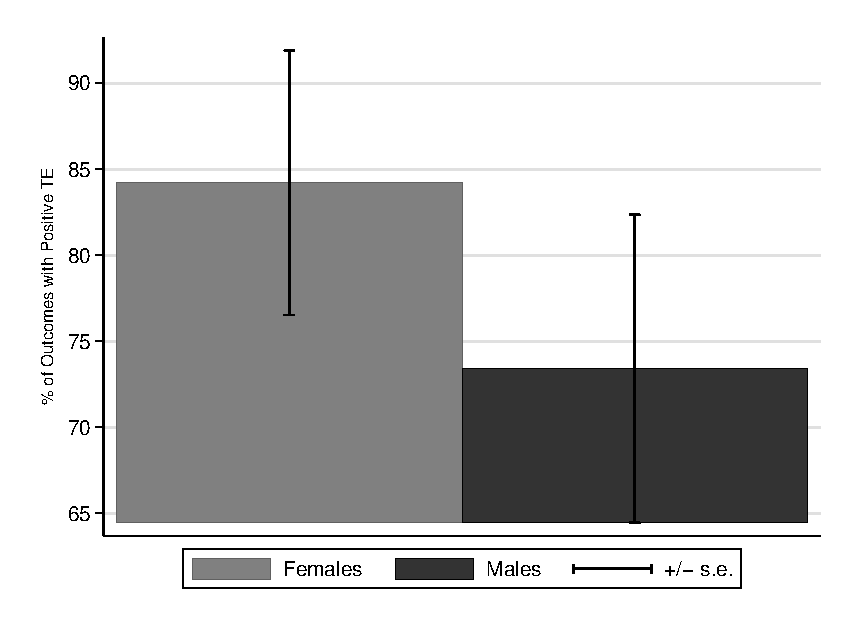
\includegraphics[width=.9\columnwidth]{output/itt_noctrl_all.eps}
\floatfoot{
\footnotesize
\noindent Note: The first two bars (ABC) compare the treatment and control groups in ABC. The third and four bars (CARE) compare the children who received center-based childcare and family education to the children who receive either family education or no treatment at all. The last two bars (ABC and CARE) pool the two previous sets of comparisons.}
\end{figure}

\noindent We can further decompose the counts in Figure~\ref{fig:ppositive} into arbitrary categories. To economize space, we present this exercise pooling ABC and CARE. That is, we decompose the effects described in the last two bars of Figure~\ref{fig:ppositive}. Figure~\ref{fig:ppositivecategory1} and Figure~\ref{fig:ppositivecategory2} present this exercise. This helps us better understand the type of outcomes in which the programs had effects. The results indicate that a large and precise fraction of effects are positive in outcomes spanning the life-cycle, from parental income to crime and including a wide variety of health categories.\\

\begin{figure}[H]
		\caption{Positively Impacted Outcomes by Category, ABC and CARE} \label{fig:ppositivecategory1}
		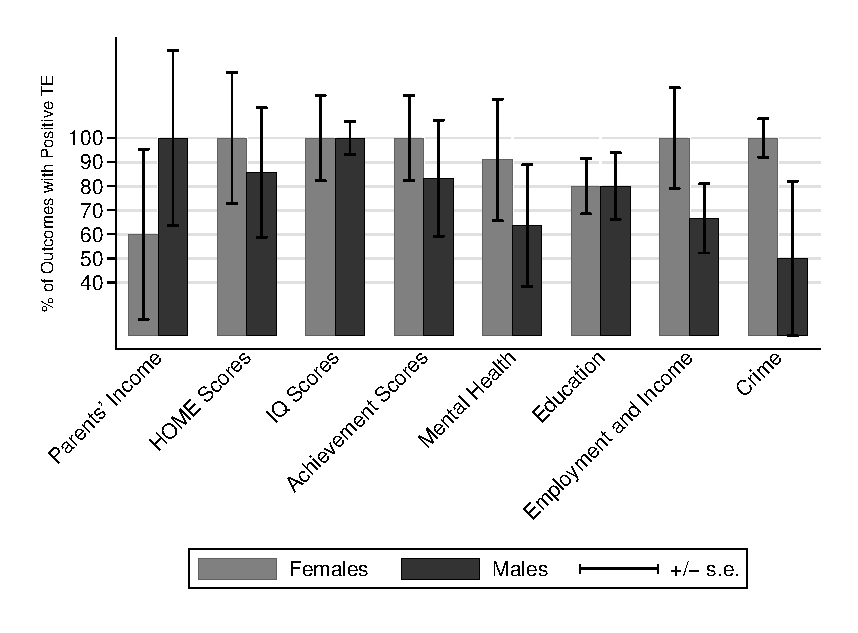
\includegraphics[width=.9\columnwidth]{output/itt_noctrl_cats1.eps}
\floatfoot{
\footnotesize
\noindent Note: For each outcome category, we compare the mean of the children who received center-based childcare in ABC and center-based childcare and family education in ABC to the mean of the children in the control group in ABC and the control and the family education treatment groups in CARE and count the number of positive comparisons.}
\end{figure}

\noindent Although the exercise in Figure~\ref{fig:ppositive}, Figure~\ref{fig:ppositivecategory1}, and Figure~\ref{fig:ppositivecategory2} is informative by itself, more rigor and more detail are necessary to inform policy-making. We present a thorough documentation of our results next. The results we present are by gender. The motivation for us to do this, is that the effects of early-childhood education program usually differ by gender \citep{Heckman_Moon_etal_2010_QE,Campbell_Conti_etal_2014_EarlyChildhoodInvestments}.\footnote{In fact, recent some studies show that the effects of exposure to different environments differ by gender. A recent example is \citet{Autor-etal_2015_Family-Disadvantage}, which includes a discussion of the related literature.} Generally, the point estimates indicate that the benefits are similar for both females and males.\\

\begin{figure}[H]
		\caption{Positively Impacted Outcomes, ABC and CARE} \label{fig:ppositivecategory2}
		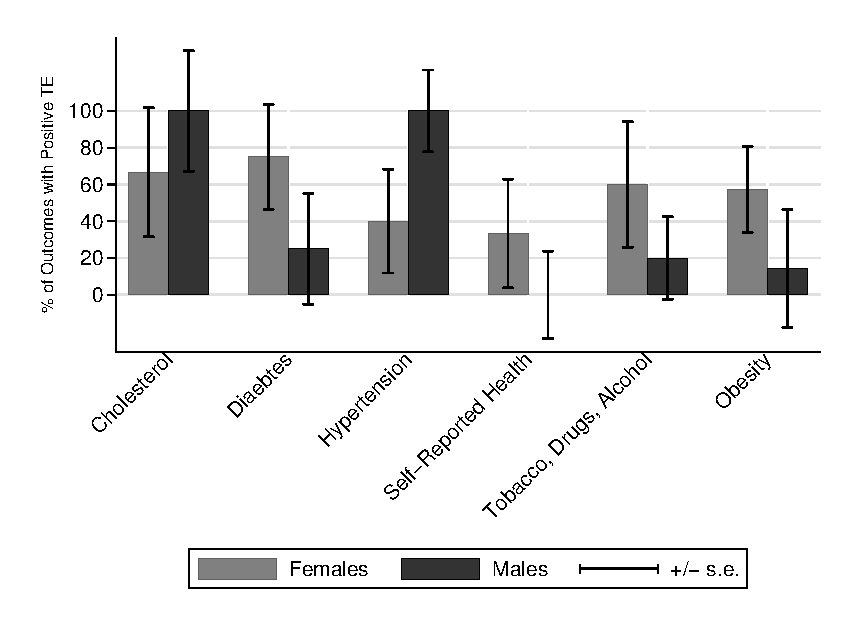
\includegraphics[width=.9\columnwidth]{output/itt_noctrl_cats2.eps}
\floatfoot{
\footnotesize
\noindent Note: For each outcome category, we compare the mean of the children who received center-based childcare in ABC and center-based childcare and family education in ABC to the mean of the children in the control group in ABC and the control and the family education treatment groups in CARE and count the number of positive comparisons.}
\end{figure}

\noindent The reminder of this section proceeds as follows. Section~\ref{section:center} presents our main results, which test the effect of the first phase of treatment. Section~\ref{section:centerfemales} focuses on females and Section~\ref{section:centermales} on males. Section~\ref{section:second} discusses the effects of the treatment's second phase.\\

\subsection{First Phase of Treatment} \label{section:center}

\noindent Our main results are based on pooling the data from ABC and CARE to test the hypothesis in \eqref{eq:ho}. That is, to test the effect of center-based childcare. We compare children who were randomly assigned to treatment in ABC and to center-based childcare and family education treatment in CARE to children who were not assigned center-based childcare in either program, correcting for program attrition and accounting for treatment substitution. The motivation for pooling the sample in this way is based on two facts: (i) the family education treatment had no substantial effect compared to the control group, providing evidence on center-based childcare being the main component causing treatment effects in CARE; and (ii) comparing the groups receiving center-based childcare to the control groups of ABC and CARE independently, provides results very similar to those we discuss here. We document these two facts in Appendix~\ref{appendix:results}.\\

\noindent By pooling ABC and CARE, we are able to test the effectiveness of center-based childcare as a policy, rather than testing the effectiveness of a program as it was implemented.\\

\subsubsection{Females} \label{section:centerfemales}

\noindent We consider a large variety of outcomes when evaluating the program in its entirety. To illustrate how our program attrition and treatment substitution, we present a summary of results in Tables~\ref{tab:ate_female_main1} and \ref{tab:ate_female_main2}. For each outcome, we present eight estimates. To illustrate how we interpret each estimate, consider high school graduation at age 30. We discuss the other outcomes afterward.\\

\noindent Column~(1) displays the mean difference in graduation between children assigned and not assigned to receive center-based childcare. This difference amounts to 20 percentage points. In column~(2) we present this difference controlling for a set of variables and accounting for program attrition.\footnote{See Appendix~\ref{appendix:controls} for our procedure for selecting controls.} In this case, the estimate remains practically unchanged. This is generally the case for all the estimates we consider, so we will restrict our discussion to estimates in which we include controls and account for program attrition.\\

\noindent The estimates in column (2) correspond to our first policy question: What is the effect of center-based childcare relative to the mix of alternatives at implementation? That is, we do not fix alternative preschools take-up.\\

\noindent Columns (4) and (5) provide estimates where the treatment substitute is fixed. Specifically, they assess the more policy-relevant question: What is the effect of center-based childcare relative to a counterfactual where the child receives no alternative preschool? In column (4), we compare the adjusted mean of children assigned and not assigned to center-based childcare. For children not assigned to center-based childcare, we restrict the sample to those who did not enroll in any alternative preschools. Compared to that of column (1), the effect almost doubles. To take into account possible selection into preschool alternatives, we consider a matching strategy.\footnote{We parameterize the matching using an Epanechnikov kernel-weight approach. Results are not sensitive to matching using nearest neighbor or propensity score matching.} If selection into preschool is based on observed characteristics, column (5) provides a selection-corrected estimate, relative to the estimate in column (3). The difference between (3) and (5) is economically sizable, as it amounts to a 6 percentage point decrease in high school graduation. This difference suggests that parents select on potential gains when enrolling their female children into preschool alternatives. However, estimates in both columns (3) and (5) suggest that fixing children to an alternative of no preschool implies a sizable increase in the estimated treatment effect of center-based childcare. \\

\noindent Columns (7) and (8) present estimates that inform another policy question: What is the effect of center-based childcare relative to a counterfactual where the child receives care from a fixed preschool alternative? The alternative we fixed is a non-program preschool, which was high but  presumably lower quality than ABC or CARE and started treatment later, from ages 3 to 5 (see Appendix~\ref{appendix:background}, where we document this and argue that the alternative preschools were roughly homogeneous in quality). Therefore, this experiment consists of evaluating high-quality center-based childcare to an alternative of lower quality and intensity. As expected, the estimates decrease compared to the estimates in which children receive no center-based treatment. As before, the comparison between the estimates in columns (6) and column (8) suggest that parents select on potential gains. This reinforces the claim we make throughout the paper: evaluation estimates depend substantially on the counterfactual.\\

\noindent Next we discuss the reminder of outcomes in Table~\ref{tab:ate_female_main1} and Table~\ref{tab:ate_female_main2}. For cognition, we present treatment effects at age 12 because it is the latest age at which results on this outcome are available for both programs---the measure we use is the Wechsler Intelligence Scale for Children. Independently of the treatment substitution correction, the effect amounts to half standard deviation of the population's distribution. This effect is sizable, especially considering that early childhood education programs have been criticized for the fade out of their treatment effects on cognition \citep{Elango_Hojman_etal_2015_Early-Edu}. This phenomenon usually occurs at elementary school entry, way before age 12. For ABC, actually, we find sizable effects at age 21, for which we have cognition tests available (see Appendix~\ref{appendix:results}). For achievement at age 8, the effects are sizable as well. The effects accounting for treatment substitution are 3 points above the results not doing so; this amounts to more than 2/3 of the population standard deviation.\\

\noindent The labor market outcomes for women substantially improved. When not accounting for treatment substitution, women's employment increases 11\%, welfare dependency decreases by almost 1,000 yearly dollars (2014 USD), and labor income increases by bearly \$700 (2014 USD). When accounting for treatment substitution these results strengthen, although they lose statistical significance. The programs also reduce criminal activity, especially the number of misdemeanor arrests. When (not) accounting for treatment substitution, the program causes a decrease of (1.08) 2.28 mismemeanor arrests by age 34.\\

\noindent For females, the program does not have many statistically precise effects on health outcomes. However, these effects help verify the pattern we describe for high-school graduation, which almost all outcomes satisfy: (i) a socially positive effect of the programs, although not statistically significant for every outcome; (ii) controlling for background characteristics and correcting for program attrition has little effect on our estimates; (iii) when fixing the counterfactual to no alternative preschool, the effect of center-based childcare with respect to the counterfactual strengthens; (iv) likewise, the effect weakens when fixing the counterfactual to a lower-quality preschool; and (v) the estimates in which we correct for potential selection shrink in absolute value, but the pattern in (iii) and (iv) persists.\\

\noindent To conclude our discussion of results for female outcomes, we summarize the total number of socially positive effects that the program has on the multiple outcomes we consider in Table~\ref{tab:counts_female}.\footnote{By ``socially positive'' we mean that we reverse the effects for outcomes such as crime or obesity when counting the effects of the program.} These outcomes represent multiple measures of human development from birth to adulthood and go beyond what we present in Table~\ref{tab:ate_female_main1} and Table~\ref{tab:ate_female_main2}---see Section~\ref{section:data} and Appendix~\ref{appendix:data} for a thorough discussion on all the outcomes.\\ 

\noindent The results in Table~\ref{tab:counts_female} are compelling. Our count statistic shows that more than 78\% of all treatment effect estimates we present are positive; 37\% are positive and significant. We test the first percentage against the null hypothesis of at most 50\% of the outcomes having a positive effect and the second against the null hypothesis of at most 10\% of the outcomes being positive and significant. We strongly reject both hypotheses---the $p$-value's are in parentheses underneath the counts in Table~\ref{tab:counts_female}. 

\noindent When we fix to no preschool alternative the children who were not randomly assigned to receive center-based childcare, our count statistic shows that nearly 50\% of the effects are positive and significant at the 10\% level. For these estimates, we reject the null hypothesis of at most 10\% of the effects being significant at the 10\% level.\\

\begin{table}[H]
\captionsetup{singlelinecheck=false,justification=centering}
\caption{ABC/CARE Average Treatment Effects, Females \\ Education, Employment, and Crime \label{tab:ate_female_main1}}

  \begin{threeparttable}
  \begin{tabular}{cccccccccc}
  \hline\hline

     &  & \scriptsize{(1)} & \scriptsize{(2)} & \scriptsize{(3)} & \scriptsize{(4)} & \scriptsize{(5)} & \scriptsize{(6)} & \scriptsize{(7)} & \scriptsize{(8)} \\  

     &  &  &  & \mc{3}{c}{\scriptsize{$P=0$}} & \mc{3}{c}{\scriptsize{$P=1$}} \\ 
    \cmidrule(lr){5-7} \cmidrule(lr){8-10} 

    \scriptsize{Variable} & \scriptsize{Age} & \scriptsize{ITT} & \scriptsize{ITT$|X,W$} & \scriptsize{ITT} & \scriptsize{ITT$|X,W$} & \scriptsize{KE$|X,W$} & \scriptsize{ITT} & \scriptsize{ITT$|X,W$} & \scriptsize{KE$|X,W$} \\ 
    \hline  

    \mc{1}{l}{\scriptsize{Std. IQ Test}} & \mc{1}{c}{\scriptsize{12}} & \mc{1}{c}{\scriptsize{8.259}} & \mc{1}{c}{\scriptsize{10.271}} & \mc{1}{c}{\scriptsize{8.457}} & \mc{1}{c}{\scriptsize{11.647}} & \mc{1}{c}{\scriptsize{7.881}} & \mc{1}{c}{\scriptsize{8.167}} & \mc{1}{c}{\scriptsize{9.877}} & \mc{1}{c}{\scriptsize{7.186}} \\  

     &  & \mc{1}{c}{\scriptsize{\textbf{(0.000)}}} & \mc{1}{c}{\scriptsize{\textbf{(0.000)}}} & \mc{1}{c}{\scriptsize{\textbf{(0.000)}}} & \mc{1}{c}{\scriptsize{\textbf{(0.020)}}} & \mc{1}{c}{\scriptsize{\textbf{(0.000)}}} & \mc{1}{c}{\scriptsize{\textbf{(0.000)}}} & \mc{1}{c}{\scriptsize{\textbf{(0.000)}}} & \mc{1}{c}{\scriptsize{\textbf{(0.020)}}} \\  

    \mc{1}{l}{\scriptsize{Std. Achv.  Test}} & \mc{1}{c}{\scriptsize{8}} & \mc{1}{c}{\scriptsize{5.404}} & \mc{1}{c}{\scriptsize{8.690}} & \mc{1}{c}{\scriptsize{8.100}} & \mc{1}{c}{\scriptsize{15.721}} & \mc{1}{c}{\scriptsize{11.046}} & \mc{1}{c}{\scriptsize{4.382}} & \mc{1}{c}{\scriptsize{7.048}} & \mc{1}{c}{\scriptsize{5.065}} \\  

     &  & \mc{1}{c}{\scriptsize{\textbf{(0.020)}}} & \mc{1}{c}{\scriptsize{\textbf{(0.000)}}} & \mc{1}{c}{\scriptsize{\textbf{(0.020)}}} & \mc{1}{c}{\scriptsize{\textbf{(0.000)}}} & \mc{1}{c}{\scriptsize{\textbf{(0.000)}}} & \mc{1}{c}{\scriptsize{\textbf{(0.059)}}} & \mc{1}{c}{\scriptsize{\textbf{(0.000)}}} & \mc{1}{c}{\scriptsize{\textbf{(0.020)}}} \\  

    \mc{1}{l}{\scriptsize{Graduated High School}} & \mc{1}{c}{\scriptsize{30}} & \mc{1}{c}{\scriptsize{0.213}} & \mc{1}{c}{\scriptsize{0.224}} & \mc{1}{c}{\scriptsize{0.367}} & \mc{1}{c}{\scriptsize{0.411}} & \mc{1}{c}{\scriptsize{0.352}} & \mc{1}{c}{\scriptsize{0.142}} & \mc{1}{c}{\scriptsize{0.146}} & \mc{1}{c}{\scriptsize{0.090}} \\  

     &  & \mc{1}{c}{\scriptsize{\textbf{(0.039)}}} & \mc{1}{c}{\scriptsize{\textbf{(0.039)}}} & \mc{1}{c}{\scriptsize{\textbf{(0.000)}}} & \mc{1}{c}{\scriptsize{\textbf{(0.000)}}} & \mc{1}{c}{\scriptsize{\textbf{(0.020)}}} & \mc{1}{c}{\scriptsize{(0.118)}} & \mc{1}{c}{\scriptsize{\textbf{(0.098)}}} & \mc{1}{c}{\scriptsize{(0.196)}} \\  

    \mc{1}{l}{\scriptsize{Years of Edu.}} & \mc{1}{c}{\scriptsize{30}} & \mc{1}{c}{\scriptsize{1.474}} & \mc{1}{c}{\scriptsize{1.696}} & \mc{1}{c}{\scriptsize{1.967}} & \mc{1}{c}{\scriptsize{2.247}} & \mc{1}{c}{\scriptsize{1.291}} & \mc{1}{c}{\scriptsize{1.244}} & \mc{1}{c}{\scriptsize{1.357}} & \mc{1}{c}{\scriptsize{0.993}} \\  

     &  & \mc{1}{c}{\scriptsize{\textbf{(0.020)}}} & \mc{1}{c}{\scriptsize{\textbf{(0.020)}}} & \mc{1}{c}{\scriptsize{\textbf{(0.020)}}} & \mc{1}{c}{\scriptsize{\textbf{(0.020)}}} & \mc{1}{c}{\scriptsize{(0.118)}} & \mc{1}{c}{\scriptsize{\textbf{(0.020)}}} & \mc{1}{c}{\scriptsize{\textbf{(0.020)}}} & \mc{1}{c}{\scriptsize{\textbf{(0.078)}}} \\  

    \mc{1}{l}{\scriptsize{Labor Income}} & \mc{1}{c}{\scriptsize{30}} & \mc{1}{c}{\scriptsize{928}} & \mc{1}{c}{\scriptsize{677}} & \mc{1}{c}{\scriptsize{1,433}} & \mc{1}{c}{\scriptsize{637}} & \mc{1}{c}{\scriptsize{1,391}} & \mc{1}{c}{\scriptsize{691}} & \mc{1}{c}{\scriptsize{308}} & \mc{1}{c}{\scriptsize{300}} \\  

     &  & \mc{1}{c}{\scriptsize{(0.314)}} & \mc{1}{c}{\scriptsize{(0.412)}} & \mc{1}{c}{\scriptsize{(0.353)}} & \mc{1}{c}{\scriptsize{(0.471)}} & \mc{1}{c}{\scriptsize{(0.235)}} & \mc{1}{c}{\scriptsize{(0.392)}} & \mc{1}{c}{\scriptsize{(0.392)}} & \mc{1}{c}{\scriptsize{(0.451)}} \\  

    \mc{1}{l}{\scriptsize{Public-Transfer Income}} & \mc{1}{c}{\scriptsize{30}} & \mc{1}{c}{\scriptsize{-884}} & \mc{1}{c}{\scriptsize{-951}} & \mc{1}{c}{\scriptsize{-980}} & \mc{1}{c}{\scriptsize{-971}} & \mc{1}{c}{\scriptsize{-508}} & \mc{1}{c}{\scriptsize{-839}} & \mc{1}{c}{\scriptsize{-964}} & \mc{1}{c}{\scriptsize{-676}} \\  

     &  & \mc{1}{c}{\scriptsize{\textbf{(0.059)}}} & \mc{1}{c}{\scriptsize{\textbf{(0.098)}}} & \mc{1}{c}{\scriptsize{\textbf{(0.020)}}} & \mc{1}{c}{\scriptsize{\textbf{(0.098)}}} & \mc{1}{c}{\scriptsize{(0.216)}} & \mc{1}{c}{\scriptsize{(0.118)}} & \mc{1}{c}{\scriptsize{(0.118)}} & \mc{1}{c}{\scriptsize{(0.157)}} \\  

    \mc{1}{l}{\scriptsize{Employed}} & \mc{1}{c}{\scriptsize{30}} & \mc{1}{c}{\scriptsize{0.110}} & \mc{1}{c}{\scriptsize{0.111}} & \mc{1}{c}{\scriptsize{0.233}} & \mc{1}{c}{\scriptsize{0.235}} & \mc{1}{c}{\scriptsize{0.204}} & \mc{1}{c}{\scriptsize{0.052}} & \mc{1}{c}{\scriptsize{0.056}} & \mc{1}{c}{\scriptsize{0.037}} \\  

     &  & \mc{1}{c}{\scriptsize{\textbf{(0.078)}}} & \mc{1}{c}{\scriptsize{\textbf{(0.098)}}} & \mc{1}{c}{\scriptsize{\textbf{(0.000)}}} & \mc{1}{c}{\scriptsize{\textbf{(0.078)}}} & \mc{1}{c}{\scriptsize{(0.157)}} & \mc{1}{c}{\scriptsize{(0.314)}} & \mc{1}{c}{\scriptsize{(0.255)}} & \mc{1}{c}{\scriptsize{(0.373)}} \\  

    \mc{1}{l}{\scriptsize{Total Felony Arrests}} & \mc{1}{c}{\scriptsize{Mid-30s}} & \mc{1}{c}{\scriptsize{-0.266}} & \mc{1}{c}{\scriptsize{-0.337}} & \mc{1}{c}{\scriptsize{-0.763}} & \mc{1}{c}{\scriptsize{-1.004}} & \mc{1}{c}{\scriptsize{-1.046}} & \mc{1}{c}{\scriptsize{-0.050}} & \mc{1}{c}{\scriptsize{-0.078}} & \mc{1}{c}{\scriptsize{-0.021}} \\  

     &  & \mc{1}{c}{\scriptsize{(0.157)}} & \mc{1}{c}{\scriptsize{(0.137)}} & \mc{1}{c}{\scriptsize{\textbf{(0.098)}}} & \mc{1}{c}{\scriptsize{(0.137)}} & \mc{1}{c}{\scriptsize{(0.118)}} & \mc{1}{c}{\scriptsize{(0.255)}} & \mc{1}{c}{\scriptsize{(0.196)}} & \mc{1}{c}{\scriptsize{(0.392)}} \\  

    \mc{1}{l}{\scriptsize{Total Misdemeanor Arrests}} & \mc{1}{c}{\scriptsize{Mid-30s}} & \mc{1}{c}{\scriptsize{-0.918}} & \mc{1}{c}{\scriptsize{-1.081}} & \mc{1}{c}{\scriptsize{-1.939}} & \mc{1}{c}{\scriptsize{-2.437}} & \mc{1}{c}{\scriptsize{-2.284}} & \mc{1}{c}{\scriptsize{-0.475}} & \mc{1}{c}{\scriptsize{-0.556}} & \mc{1}{c}{\scriptsize{-0.224}} \\  

     &  & \mc{1}{c}{\scriptsize{\textbf{(0.020)}}} & \mc{1}{c}{\scriptsize{\textbf{(0.078)}}} & \mc{1}{c}{\scriptsize{\textbf{(0.059)}}} & \mc{1}{c}{\scriptsize{\textbf{(0.078)}}} & \mc{1}{c}{\scriptsize{\textbf{(0.000)}}} & \mc{1}{c}{\scriptsize{(0.137)}} & \mc{1}{c}{\scriptsize{(0.118)}} & \mc{1}{c}{\scriptsize{(0.196)}} \\  

    \mc{1}{l}{\scriptsize{Total Years Incarcerated}} & \mc{1}{c}{\scriptsize{30}} & \mc{1}{c}{\scriptsize{-0.020}} & \mc{1}{c}{\scriptsize{-0.014}} &  &  &  & \mc{1}{c}{\scriptsize{-0.031}} & \mc{1}{c}{\scriptsize{-0.025}} & \mc{1}{c}{\scriptsize{-0.021}} \\  

     &  & \mc{1}{c}{\scriptsize{\textbf{(0.059)}}} & \mc{1}{c}{\scriptsize{\textbf{(0.078)}}} &  &  &  & \mc{1}{c}{\scriptsize{\textbf{(0.078)}}} & \mc{1}{c}{\scriptsize{\textbf{(0.078)}}} & \mc{1}{c}{\scriptsize{\textbf{(0.078)}}} \\  

  \hline\hline
  \end{tabular}
    \begin{tablenotes}
    \scriptsize
    \item 
Note: This table displays various estimates of the treatment effect of ABC/CARE's center-based care.
Column (1) displays the ITT, without accounting for any controls.
Column (2) displays the ITT conditioning on vector of controls, $X$, consisting of APGAR scores 1 
minute after birth, an indicator for the subject being born prematurely, and an indicator for the 
father being home at baseline. We also apply IPW weights, $W$, to account for attrition.
Columns (3)--(4) are analogous to columns (1)--(2), but we restrict the control sample to subjects
who did not enroll in any alternative care.
Column (5) displys the matching estimate, where we use the Mahalanobis metric and Epanechnikov kernel
to match on controls $X$ listed above, and restrict the control sample to subjects who did not enroll
in any alternative care. Additionally, we apply IPW weights, $W$.
Columns (6)--(8) are analogous to Columns (3)--(5), except we restrict the control sample to subejcts
who did enroll in alternative care. 
Numbers in parentheses represent the $p$-value from a single hypothesis test, and are obtained from 
the empirical bootstrap distribution generated by 200 resamples of the original data. 
Bold $p$-values indicate significance at the 10\% level.
Blank point estimates indicate that we are unable to obtain estimates due to a lack of support in the data. 

    \end{tablenotes}
  \end{threeparttable}

\end{table}
\begin{table}[H]
\captionsetup{singlelinecheck=false,justification=centering}
\caption{ABC/CARE Average Treatment Effects, Females \\ Health Biomarkers \label{tab:ate_female_main2}}

  \begin{threeparttable}
  \begin{tabular}{cccccccccc}
  \hline\hline

     &  & \scriptsize{(1)} & \scriptsize{(2)} & \scriptsize{(3)} & \scriptsize{(4)} & \scriptsize{(5)} & \scriptsize{(6)} & \scriptsize{(7)} & \scriptsize{(8)} \\  

     &  &  &  & \mc{3}{c}{\scriptsize{$P=0$}} & \mc{3}{c}{\scriptsize{$P=1$}} \\ 
    \cmidrule(lr){5-7} \cmidrule(lr){8-10} 

    \scriptsize{Variable} & \scriptsize{Age} & \scriptsize{ITT} & \scriptsize{ITT$|X,W$} & \scriptsize{ITT} & \scriptsize{ITT$|X,W$} & \scriptsize{KE$|X,W$} & \scriptsize{ITT} & \scriptsize{ITT$|X,W$} & \scriptsize{KE$|X,W$} \\ 
    \hline  

    \mc{1}{l}{\scriptsize{Systolic Blood Pressure (mm Hg)}} & \mc{1}{c}{\scriptsize{Mid-30s}} & \mc{1}{c}{\scriptsize{-0.987}} & \mc{1}{c}{\scriptsize{-1.657}} & \mc{1}{c}{\scriptsize{3.474}} & \mc{1}{c}{\scriptsize{7.882}} & \mc{1}{c}{\scriptsize{4.088}} & \mc{1}{c}{\scriptsize{-2.805}} & \mc{1}{c}{\scriptsize{-3.455}} & \mc{1}{c}{\scriptsize{-1.778}} \\  

     &  & \mc{1}{c}{\scriptsize{(0.373)}} & \mc{1}{c}{\scriptsize{(0.353)}} & \mc{1}{c}{\scriptsize{(0.725)}} & \mc{1}{c}{\scriptsize{(0.902)}} & \mc{1}{c}{\scriptsize{(0.549)}} & \mc{1}{c}{\scriptsize{(0.275)}} & \mc{1}{c}{\scriptsize{(0.275)}} & \mc{1}{c}{\scriptsize{(0.235)}} \\  

    \mc{1}{l}{\scriptsize{Diastolic Blood Pressure (mm Hg)}} & \mc{1}{c}{\scriptsize{Mid-30s}} & \mc{1}{c}{\scriptsize{1.575}} & \mc{1}{c}{\scriptsize{1.376}} & \mc{1}{c}{\scriptsize{5.210}} & \mc{1}{c}{\scriptsize{9.353}} & \mc{1}{c}{\scriptsize{5.068}} & \mc{1}{c}{\scriptsize{0.095}} & \mc{1}{c}{\scriptsize{-0.057}} & \mc{1}{c}{\scriptsize{1.986}} \\  

     &  & \mc{1}{c}{\scriptsize{(0.608)}} & \mc{1}{c}{\scriptsize{(0.569)}} & \mc{1}{c}{\scriptsize{(0.882)}} & \mc{1}{c}{\scriptsize{(0.961)}} & \mc{1}{c}{\scriptsize{(0.588)}} & \mc{1}{c}{\scriptsize{(0.373)}} & \mc{1}{c}{\scriptsize{(0.431)}} & \mc{1}{c}{\scriptsize{(0.471)}} \\  

    \mc{1}{l}{\scriptsize{Prehypertension}} & \mc{1}{c}{\scriptsize{Mid-30s}} & \mc{1}{c}{\scriptsize{-0.156}} & \mc{1}{c}{\scriptsize{-0.163}} & \mc{1}{c}{\scriptsize{-0.079}} & \mc{1}{c}{\scriptsize{0.118}} & \mc{1}{c}{\scriptsize{-0.191}} & \mc{1}{c}{\scriptsize{-0.187}} & \mc{1}{c}{\scriptsize{-0.222}} & \mc{1}{c}{\scriptsize{-0.199}} \\  

     &  & \mc{1}{c}{\scriptsize{(0.118)}} & \mc{1}{c}{\scriptsize{(0.118)}} & \mc{1}{c}{\scriptsize{(0.333)}} & \mc{1}{c}{\scriptsize{(0.725)}} & \mc{1}{c}{\scriptsize{\textbf{(0.059)}}} & \mc{1}{c}{\scriptsize{\textbf{(0.078)}}} & \mc{1}{c}{\scriptsize{\textbf{(0.039)}}} & \mc{1}{c}{\scriptsize{(0.118)}} \\  

    \mc{1}{l}{\scriptsize{Hypertension}} & \mc{1}{c}{\scriptsize{Mid-30s}} & \mc{1}{c}{\scriptsize{0.197}} & \mc{1}{c}{\scriptsize{0.180}} & \mc{1}{c}{\scriptsize{0.202}} & \mc{1}{c}{\scriptsize{0.352}} & \mc{1}{c}{\scriptsize{0.159}} & \mc{1}{c}{\scriptsize{0.195}} & \mc{1}{c}{\scriptsize{0.161}} & \mc{1}{c}{\scriptsize{0.201}} \\  

     &  & \mc{1}{c}{\scriptsize{(0.980)}} & \mc{1}{c}{\scriptsize{(0.941)}} & \mc{1}{c}{\scriptsize{(0.843)}} & \mc{1}{c}{\scriptsize{(1.000)}} & \mc{1}{c}{\scriptsize{(0.588)}} & \mc{1}{c}{\scriptsize{(0.961)}} & \mc{1}{c}{\scriptsize{(0.843)}} & \mc{1}{c}{\scriptsize{(0.784)}} \\  

    \mc{1}{l}{\scriptsize{High-Density Lipoprotein Chol. (mg/dL)}} & \mc{1}{c}{\scriptsize{Mid-30s}} & \mc{1}{c}{\scriptsize{3.690}} & \mc{1}{c}{\scriptsize{2.173}} & \mc{1}{c}{\scriptsize{9.984}} & \mc{1}{c}{\scriptsize{6.502}} & \mc{1}{c}{\scriptsize{10.334}} & \mc{1}{c}{\scriptsize{1.126}} & \mc{1}{c}{\scriptsize{0.167}} & \mc{1}{c}{\scriptsize{3.222}} \\  

     &  & \mc{1}{c}{\scriptsize{(0.137)}} & \mc{1}{c}{\scriptsize{(0.216)}} & \mc{1}{c}{\scriptsize{\textbf{(0.000)}}} & \mc{1}{c}{\scriptsize{\textbf{(0.078)}}} & \mc{1}{c}{\scriptsize{\textbf{(0.000)}}} & \mc{1}{c}{\scriptsize{(0.275)}} & \mc{1}{c}{\scriptsize{(0.431)}} & \mc{1}{c}{\scriptsize{(0.216)}} \\  

    \mc{1}{l}{\scriptsize{Dyslipidemia}} & \mc{1}{c}{\scriptsize{Mid-30s}} & \mc{1}{c}{\scriptsize{0.034}} & \mc{1}{c}{\scriptsize{0.063}} & \mc{1}{c}{\scriptsize{-0.004}} & \mc{1}{c}{\scriptsize{0.044}} & \mc{1}{c}{\scriptsize{0.013}} & \mc{1}{c}{\scriptsize{0.050}} & \mc{1}{c}{\scriptsize{0.073}} & \mc{1}{c}{\scriptsize{0.043}} \\  

     &  & \mc{1}{c}{\scriptsize{(0.725)}} & \mc{1}{c}{\scriptsize{(0.804)}} & \mc{1}{c}{\scriptsize{(0.451)}} & \mc{1}{c}{\scriptsize{(0.588)}} & \mc{1}{c}{\scriptsize{(0.333)}} & \mc{1}{c}{\scriptsize{(0.843)}} & \mc{1}{c}{\scriptsize{(0.863)}} & \mc{1}{c}{\scriptsize{(0.588)}} \\  

    \mc{1}{l}{\scriptsize{Hemoglobin Level (\%)}} & \mc{1}{c}{\scriptsize{Mid-30s}} & \mc{1}{c}{\scriptsize{-0.188}} & \mc{1}{c}{\scriptsize{-0.264}} & \mc{1}{c}{\scriptsize{-0.173}} & \mc{1}{c}{\scriptsize{-0.176}} & \mc{1}{c}{\scriptsize{-0.146}} & \mc{1}{c}{\scriptsize{-0.194}} & \mc{1}{c}{\scriptsize{-0.245}} & \mc{1}{c}{\scriptsize{-0.202}} \\  

     &  & \mc{1}{c}{\scriptsize{(0.176)}} & \mc{1}{c}{\scriptsize{(0.157)}} & \mc{1}{c}{\scriptsize{\textbf{(0.039)}}} & \mc{1}{c}{\scriptsize{\textbf{(0.020)}}} & \mc{1}{c}{\scriptsize{\textbf{(0.039)}}} & \mc{1}{c}{\scriptsize{(0.196)}} & \mc{1}{c}{\scriptsize{(0.176)}} & \mc{1}{c}{\scriptsize{(0.176)}} \\  

    \mc{1}{l}{\scriptsize{Prediabetes}} & \mc{1}{c}{\scriptsize{Mid-30s}} & \mc{1}{c}{\scriptsize{0.093}} & \mc{1}{c}{\scriptsize{0.044}} & \mc{1}{c}{\scriptsize{0.045}} & \mc{1}{c}{\scriptsize{-0.035}} & \mc{1}{c}{\scriptsize{0.069}} & \mc{1}{c}{\scriptsize{0.113}} & \mc{1}{c}{\scriptsize{0.084}} & \mc{1}{c}{\scriptsize{0.039}} \\  

     &  & \mc{1}{c}{\scriptsize{(0.725)}} & \mc{1}{c}{\scriptsize{(0.647)}} & \mc{1}{c}{\scriptsize{(0.667)}} & \mc{1}{c}{\scriptsize{(0.431)}} & \mc{1}{c}{\scriptsize{(0.569)}} & \mc{1}{c}{\scriptsize{(0.824)}} & \mc{1}{c}{\scriptsize{(0.725)}} & \mc{1}{c}{\scriptsize{(0.529)}} \\  

    \mc{1}{l}{\scriptsize{Diabetes}} & \mc{1}{c}{\scriptsize{Mid-30s}} & \mc{1}{c}{\scriptsize{-0.053}} & \mc{1}{c}{\scriptsize{-0.073}} &  &  &  & \mc{1}{c}{\scriptsize{-0.074}} & \mc{1}{c}{\scriptsize{-0.091}} & \mc{1}{c}{\scriptsize{-0.081}} \\  

     &  & \mc{1}{c}{\scriptsize{\textbf{(0.059)}}} & \mc{1}{c}{\scriptsize{\textbf{(0.020)}}} &  &  &  & \mc{1}{c}{\scriptsize{\textbf{(0.059)}}} & \mc{1}{c}{\scriptsize{\textbf{(0.039)}}} & \mc{1}{c}{\scriptsize{\textbf{(0.020)}}} \\  

    \mc{1}{l}{\scriptsize{Vitamin D Deficiency}} & \mc{1}{c}{\scriptsize{Mid-30s}} & \mc{1}{c}{\scriptsize{-0.050}} & \mc{1}{c}{\scriptsize{-0.021}} & \mc{1}{c}{\scriptsize{-0.079}} & \mc{1}{c}{\scriptsize{-0.070}} & \mc{1}{c}{\scriptsize{-0.025}} & \mc{1}{c}{\scriptsize{-0.039}} & \mc{1}{c}{\scriptsize{-0.007}} & \mc{1}{c}{\scriptsize{-0.021}} \\  

     &  & \mc{1}{c}{\scriptsize{(0.431)}} & \mc{1}{c}{\scriptsize{(0.490)}} & \mc{1}{c}{\scriptsize{(0.353)}} & \mc{1}{c}{\scriptsize{(0.353)}} & \mc{1}{c}{\scriptsize{(0.275)}} & \mc{1}{c}{\scriptsize{(0.373)}} & \mc{1}{c}{\scriptsize{(0.490)}} & \mc{1}{c}{\scriptsize{(0.373)}} \\  

  \hline\hline
  \end{tabular}
    \begin{tablenotes}
    \scriptsize
    \item 
Note: This table displays various estimates of the treatment effect of ABC/CARE's center-based care.
Column (1) displays the ITT, without accounting for any controls.
Column (2) displays the ITT conditioning on vector of controls, $X$, consisting of APGAR scores 1 
minute after birth, an indicator for the subject being born prematurely, and an indicator for the 
father being home at baseline. We also apply IPW weights, $W$, to account for attrition.
Columns (3)--(4) are analogous to columns (1)--(2), but we restrict the control sample to subjects
who did not enroll in any alternative care.
Column (5) displys the matching estimate, where we use the Mahalanobis metric and Epanechnikov kernel
to match on controls $X$ listed above, and restrict the control sample to subjects who did not enroll
in any alternative care. Additionally, we apply IPW weights, $W$.
Columns (6)--(8) are analogous to Columns (3)--(5), except we restrict the control sample to subejcts
who did enroll in alternative care. 
Numbers in parentheses represent the $p$-value from a single hypothesis test, and are obtained from 
the empirical bootstrap distribution generated by 200 resamples of the original data. 
Bold $p$-values indicate significance at the 10\% level.
Blank point estimates indicate that we are unable to obtain estimates due to a lack of support in the data. 

    \end{tablenotes}
  \end{threeparttable}

\end{table}
  \begin{tabular}{ccccccccc}
  \toprule

     & \scriptsize{(1)} & \scriptsize{(2)} & \scriptsize{(3)} & \scriptsize{(4)} & \scriptsize{(5)} & \scriptsize{(6)} & \scriptsize{(7)} & \scriptsize{(8)} \\ 
    \midrule  

    \mc{1}{l}{\scriptsize{\% Pos. TE}} & \mc{1}{c}{\scriptsize{79}} & \mc{1}{c}{\scriptsize{73}} & \mc{1}{c}{\scriptsize{83}} & \mc{1}{c}{\scriptsize{84}} & \mc{1}{c}{\scriptsize{85}} & \mc{1}{c}{\scriptsize{72}} & \mc{1}{c}{\scriptsize{65}} & \mc{1}{c}{\scriptsize{73}} \\  

     & \mc{1}{c}{\scriptsize{\textbf{(0.000)}}} & \mc{1}{c}{\scriptsize{\textbf{(0.000)}}} & \mc{1}{c}{\scriptsize{\textbf{(0.000)}}} & \mc{1}{c}{\scriptsize{\textbf{(0.000)}}} & \mc{1}{c}{\scriptsize{\textbf{(0.000)}}} & \mc{1}{c}{\scriptsize{\textbf{(0.000)}}} & \mc{1}{c}{\scriptsize{\textbf{(0.026)}}} & \mc{1}{c}{\scriptsize{\textbf{(0.000)}}} \\  

    \mc{1}{l}{\scriptsize{\% Pos. TE $|$ 10\% Significance}} & \mc{1}{c}{\scriptsize{36}} & \mc{1}{c}{\scriptsize{35}} & \mc{1}{c}{\scriptsize{46}} & \mc{1}{c}{\scriptsize{44}} & \mc{1}{c}{\scriptsize{44}} & \mc{1}{c}{\scriptsize{23}} & \mc{1}{c}{\scriptsize{21}} & \mc{1}{c}{\scriptsize{23}} \\  

     & \mc{1}{c}{\scriptsize{\textbf{(0.000)}}} & \mc{1}{c}{\scriptsize{\textbf{(0.000)}}} & \mc{1}{c}{\scriptsize{\textbf{(0.000)}}} & \mc{1}{c}{\scriptsize{\textbf{(0.000)}}} & \mc{1}{c}{\scriptsize{\textbf{(0.000)}}} & \mc{1}{c}{\scriptsize{\textbf{(0.092)}}} & \mc{1}{c}{\scriptsize{(0.132)}} & \mc{1}{c}{\scriptsize{(0.105)}} \\  

  \bottomrule
  \end{tabular}

\subsubsection{Males} \label{section:centermales}

\noindent To illustrate the extent of effects for males, we also present a summary of results. This is in Table~\ref{tab:ate_male_main1} and Table~\ref{tab:ate_male_main2}. There are two main differences between males and females. First, for males, outcomes of greatest policy interest such as employment and labor income exhibit a much stronger effect. Second, as we discuss below, the pattern in which the effects we present from columns (1) to (8) is not as clear as in the case of females.\\

\noindent The results for cognition and achievement are not economically sizable for males. This is recurrent finding in the literature. It is also recurrent to find much less stronger effect on high school graduation \citep{Elango_Hojman_etal_2015_Early-Edu}, although the effect on years of education at age 30 are economically and statistically significant. When not accounting for treatment substitution, the positive effect is .80 years of schooling, which more than doubles when accounting for attrition.\\

\noindent For males, correcting for self-selection in the estimates that fix the counterfactual does not consistently indicate that parents enrolled their male children into preschool alternatives based on potential gains. Instead, for some outcomes this correction points toward the opposite effect. To illustrate this, consider years of education. When fixing children to no alternative preschool, the treatment effect increases by more than 0.4 years with respect to the effect where alternative preschool is not fixed. This pattern is the same in the case for females. However, unlike females, when correcting for potential self-selection in the preschool enrollment decision, the estimate further increases remains similar in magnitude. This estimate could suggest that children with the most potential (or with the best home environment) stay at home, although the analogous estimate for females indicates that female children with the least potential (or with the worst home environment) stay at home.\\

\noindent The effects on income are large and precise. When (not) accounting for treatment substitution, they amount to (\$6,055 2014 USD) \$11,310 2014 USD at age 30. Other effects as crime and reliance on public-transfer income are not as precisely estimated as the effect on income or employment but they align in pattern and signal the socially positive effects the program had. Finally, as noted in \citet{Campbell_Conti_etal_2014_EarlyChildhoodInvestments}, the effects the program has on long-term health are substantial and go from improvements in blood pressure to decrease in self-reported drug use. As before, accounting for treatment substitution strengthens these results.\\

\noindent We also present the counts of positive effects, with a comparable inference exercise, in Table~\ref{tab:counts_male}. We reject the null hypothesis that at most 50\% of the outcomes are socially positive for any of the estimates we consider.

\begin{sidewaystable}[H]
\captionsetup{singlelinecheck=false,justification=centering}
\caption{Summary of Treatment Effects of Center-based Childcare on Males \\ Education, Employment, and Crime \label{tab:ate_male_main1}}

  \begin{threeparttable}
  \begin{tabular}{cccccccccc}
  \toprule

     &  & \footnotesize{(1)} & \footnotesize{(2)} & \footnotesize{(3)} & \footnotesize{(4)} & \footnotesize{(5)} & \footnotesize{(6)} & \footnotesize{(7)} & \footnotesize{(8)} \\  

     &  &  &  & \mc{3}{c}{\footnotesize{$P=0$}} & \mc{3}{c}{\footnotesize{$P=1$}} \\ 
    \cmidrule(lr){5-7} \cmidrule(lr){8-10} 

    \footnotesize{Variable} & \footnotesize{Age} & \footnotesize{ITT} & \footnotesize{ITT$|X,W$} & \footnotesize{ITT} & \footnotesize{ITT$|X,W$} & \footnotesize{KE$|X,W$} & \footnotesize{ITT} & \footnotesize{ITT$|X,W$} & \footnotesize{KE$|X,W$} \\ 
    \midrule

    \mc{1}{l}{\footnotesize{Std. IQ Test}} & \mc{1}{c}{\footnotesize{12}} & \mc{1}{c}{\footnotesize{2.549}} & \mc{1}{c}{\footnotesize{3.312}} & \mc{1}{c}{\footnotesize{1.613}} & \mc{1}{c}{\footnotesize{1.234}} & \mc{1}{c}{\footnotesize{-0.113}} & \mc{1}{c}{\footnotesize{2.877}} & \mc{1}{c}{\footnotesize{4.365}} & \mc{1}{c}{\footnotesize{0.694}} \\  

     &  & \mc{1}{c}{\footnotesize{\textbf{(0.098)}}} & \mc{1}{c}{\footnotesize{\textbf{(0.078)}}} & \mc{1}{c}{\footnotesize{(0.333)}} & \mc{1}{c}{\footnotesize{(0.373)}} & \mc{1}{c}{\footnotesize{(0.490)}} & \mc{1}{c}{\footnotesize{\textbf{(0.078)}}} & \mc{1}{c}{\footnotesize{\textbf{(0.039)}}} & \mc{1}{c}{\footnotesize{(0.333)}} \\  

    \mc{1}{l}{\footnotesize{Std. Achv.  Test}} & \mc{1}{c}{\footnotesize{8}} & \mc{1}{c}{\footnotesize{2.948}} & \mc{1}{c}{\footnotesize{4.501}} & \mc{1}{c}{\footnotesize{0.672}} & \mc{1}{c}{\footnotesize{1.538}} & \mc{1}{c}{\footnotesize{1.135}} & \mc{1}{c}{\footnotesize{3.728}} & \mc{1}{c}{\footnotesize{5.981}} & \mc{1}{c}{\footnotesize{3.971}} \\  

     &  & \mc{1}{c}{\footnotesize{(0.118)}} & \mc{1}{c}{\footnotesize{\textbf{(0.039)}}} & \mc{1}{c}{\footnotesize{(0.490)}} & \mc{1}{c}{\footnotesize{(0.333)}} & \mc{1}{c}{\footnotesize{(0.431)}} & \mc{1}{c}{\footnotesize{\textbf{(0.059)}}} & \mc{1}{c}{\footnotesize{\textbf{(0.000)}}} & \mc{1}{c}{\footnotesize{\textbf{(0.059)}}} \\  

    \mc{1}{l}{\footnotesize{Graduated High School}} & \mc{1}{c}{\footnotesize{30}} & \mc{1}{c}{\footnotesize{0.154}} & \mc{1}{c}{\footnotesize{0.148}} & \mc{1}{c}{\footnotesize{0.114}} & \mc{1}{c}{\footnotesize{0.076}} & \mc{1}{c}{\footnotesize{0.061}} & \mc{1}{c}{\footnotesize{0.171}} & \mc{1}{c}{\footnotesize{0.176}} & \mc{1}{c}{\footnotesize{0.098}} \\  

     &  & \mc{1}{c}{\footnotesize{\textbf{(0.078)}}} & \mc{1}{c}{\footnotesize{(0.118)}} & \mc{1}{c}{\footnotesize{(0.255)}} & \mc{1}{c}{\footnotesize{(0.294)}} & \mc{1}{c}{\footnotesize{(0.392)}} & \mc{1}{c}{\footnotesize{\textbf{(0.078)}}} & \mc{1}{c}{\footnotesize{(0.118)}} & \mc{1}{c}{\footnotesize{(0.137)}} \\  

    \mc{1}{l}{\footnotesize{Years of Edu.}} & \mc{1}{c}{\footnotesize{30}} & \mc{1}{c}{\footnotesize{1.046}} & \mc{1}{c}{\footnotesize{0.801}} & \mc{1}{c}{\footnotesize{1.643}} & \mc{1}{c}{\footnotesize{1.224}} & \mc{1}{c}{\footnotesize{1.696}} & \mc{1}{c}{\footnotesize{0.792}} & \mc{1}{c}{\footnotesize{0.640}} & \mc{1}{c}{\footnotesize{0.727}} \\  

     &  & \mc{1}{c}{\footnotesize{\textbf{(0.020)}}} & \mc{1}{c}{\footnotesize{\textbf{(0.059)}}} & \mc{1}{c}{\footnotesize{\textbf{(0.000)}}} & \mc{1}{c}{\footnotesize{\textbf{(0.020)}}} & \mc{1}{c}{\footnotesize{\textbf{(0.000)}}} & \mc{1}{c}{\footnotesize{\textbf{(0.078)}}} & \mc{1}{c}{\footnotesize{(0.118)}} & \mc{1}{c}{\footnotesize{\textbf{(0.098)}}} \\  

    \mc{1}{l}{\footnotesize{Labor Income}} & \mc{1}{c}{\footnotesize{30}} & \mc{1}{c}{\footnotesize{10,070}} & \mc{1}{c}{\footnotesize{6,055}} & \mc{1}{c}{\footnotesize{10,973}} & \mc{1}{c}{\footnotesize{7,572}} & \mc{1}{c}{\footnotesize{11,310}} & \mc{1}{c}{\footnotesize{9,675}} & \mc{1}{c}{\footnotesize{5,880}} & \mc{1}{c}{\footnotesize{9,505}} \\  

     &  & \mc{1}{c}{\footnotesize{\textbf{(0.078)}}} & \mc{1}{c}{\footnotesize{\textbf{(0.098)}}} & \mc{1}{c}{\footnotesize{\textbf{(0.078)}}} & \mc{1}{c}{\footnotesize{\textbf{(0.098)}}} & \mc{1}{c}{\footnotesize{\textbf{(0.039)}}} & \mc{1}{c}{\footnotesize{\textbf{(0.078)}}} & \mc{1}{c}{\footnotesize{\textbf{(0.078)}}} & \mc{1}{c}{\footnotesize{(0.118)}} \\  

    \mc{1}{l}{\footnotesize{Public-Transfer Income}} & \mc{1}{c}{\footnotesize{30}} & \mc{1}{c}{\footnotesize{-422}} & \mc{1}{c}{\footnotesize{-492}} & \mc{1}{c}{\footnotesize{-576}} & \mc{1}{c}{\footnotesize{-813}} & \mc{1}{c}{\footnotesize{-556}} & \mc{1}{c}{\footnotesize{-357}} & \mc{1}{c}{\footnotesize{-335}} & \mc{1}{c}{\footnotesize{-409}} \\  

     &  & \mc{1}{c}{\footnotesize{\textbf{(0.059)}}} & \mc{1}{c}{\footnotesize{\textbf{(0.098)}}} & \mc{1}{c}{\footnotesize{(0.118)}} & \mc{1}{c}{\footnotesize{(0.118)}} & \mc{1}{c}{\footnotesize{\textbf{(0.098)}}} & \mc{1}{c}{\footnotesize{\textbf{(0.078)}}} & \mc{1}{c}{\footnotesize{\textbf{(0.039)}}} & \mc{1}{c}{\footnotesize{\textbf{(0.078)}}} \\  

    \mc{1}{l}{\footnotesize{Employed}} & \mc{1}{c}{\footnotesize{30}} & \mc{1}{c}{\footnotesize{0.190}} & \mc{1}{c}{\footnotesize{0.150}} & \mc{1}{c}{\footnotesize{0.186}} & \mc{1}{c}{\footnotesize{0.087}} & \mc{1}{c}{\footnotesize{0.290}} & \mc{1}{c}{\footnotesize{0.192}} & \mc{1}{c}{\footnotesize{0.168}} & \mc{1}{c}{\footnotesize{0.311}} \\  

     &  & \mc{1}{c}{\footnotesize{\textbf{(0.000)}}} & \mc{1}{c}{\footnotesize{\textbf{(0.098)}}} & \mc{1}{c}{\footnotesize{(0.118)}} & \mc{1}{c}{\footnotesize{(0.333)}} & \mc{1}{c}{\footnotesize{\textbf{(0.020)}}} & \mc{1}{c}{\footnotesize{\textbf{(0.059)}}} & \mc{1}{c}{\footnotesize{\textbf{(0.078)}}} & \mc{1}{c}{\footnotesize{\textbf{(0.000)}}} \\  

    \mc{1}{l}{\footnotesize{Total Felony Arrests}} & \mc{1}{c}{\footnotesize{Mid-30s}} & \mc{1}{c}{\footnotesize{0.145}} & \mc{1}{c}{\footnotesize{0.236}} & \mc{1}{c}{\footnotesize{0.303}} & \mc{1}{c}{\footnotesize{0.756}} & \mc{1}{c}{\footnotesize{0.800}} & \mc{1}{c}{\footnotesize{0.069}} & \mc{1}{c}{\footnotesize{0.148}} & \mc{1}{c}{\footnotesize{0.411}} \\  

     &  & \mc{1}{c}{\footnotesize{(0.608)}} & \mc{1}{c}{\footnotesize{(0.608)}} & \mc{1}{c}{\footnotesize{(0.647)}} & \mc{1}{c}{\footnotesize{(0.784)}} & \mc{1}{c}{\footnotesize{(0.804)}} & \mc{1}{c}{\footnotesize{(0.529)}} & \mc{1}{c}{\footnotesize{(0.569)}} & \mc{1}{c}{\footnotesize{(0.686)}} \\  

    \mc{1}{l}{\footnotesize{Total Misdemeanor Arrests}} & \mc{1}{c}{\footnotesize{Mid-30s}} & \mc{1}{c}{\footnotesize{-0.686}} & \mc{1}{c}{\footnotesize{-0.584}} & \mc{1}{c}{\footnotesize{-0.823}} & \mc{1}{c}{\footnotesize{-0.781}} & \mc{1}{c}{\footnotesize{-0.821}} & \mc{1}{c}{\footnotesize{-0.621}} & \mc{1}{c}{\footnotesize{-0.554}} & \mc{1}{c}{\footnotesize{-0.319}} \\  

     &  & \mc{1}{c}{\footnotesize{\textbf{(0.039)}}} & \mc{1}{c}{\footnotesize{\textbf{(0.098)}}} & \mc{1}{c}{\footnotesize{(0.118)}} & \mc{1}{c}{\footnotesize{(0.137)}} & \mc{1}{c}{\footnotesize{(0.157)}} & \mc{1}{c}{\footnotesize{\textbf{(0.078)}}} & \mc{1}{c}{\footnotesize{\textbf{(0.098)}}} & \mc{1}{c}{\footnotesize{(0.216)}} \\  

    \mc{1}{l}{\footnotesize{Total Years Incarcerated}} & \mc{1}{c}{\footnotesize{30}} & \mc{1}{c}{\footnotesize{0.106}} & \mc{1}{c}{\footnotesize{0.185}} & \mc{1}{c}{\footnotesize{0.184}} & \mc{1}{c}{\footnotesize{0.268}} & \mc{1}{c}{\footnotesize{0.367}} & \mc{1}{c}{\footnotesize{0.066}} & \mc{1}{c}{\footnotesize{0.145}} & \mc{1}{c}{\footnotesize{0.221}} \\  

     &  & \mc{1}{c}{\footnotesize{(0.667)}} & \mc{1}{c}{\footnotesize{(0.824)}} & \mc{1}{c}{\footnotesize{(0.667)}} & \mc{1}{c}{\footnotesize{(0.804)}} & \mc{1}{c}{\footnotesize{(0.843)}} & \mc{1}{c}{\footnotesize{(0.627)}} & \mc{1}{c}{\footnotesize{(0.647)}} & \mc{1}{c}{\footnotesize{(0.843)}} \\  

  \bottomrule
  \end{tabular}
    \begin{tablenotes}
    \footnotesize
    \item 
Note: This table displays various estimates of the treatment effect of ABC/CARE's center-based care.
Column (1) displays the ITT, without accounting for any controls.
Column (2) displays the ITT conditioning on vector of controls, $X$, consisting of Apgar scores 1 minute and 5 minutes after birth, the HRI index, maternal IQ,
an indicator for having a grandmother residing in the same county, and an index for the number
of relatives living in the same household. We also apply IPW weights, $W$, to account for attrition.
Columns (3)--(4) are analogous to columns (1)--(2), but we restrict the control sample to subjects
who did not enroll in any alternative care.
Column (5) displays the matching estimate, where we use the Mahalanobis metric and Epanechnikov kernel
to match on controls $X$ listed above, and restrict the control sample to subjects who did not enroll
in any alternative care. Additionally, we apply IPW weights, $W$.
Columns (6)--(8) are analogous to Columns (3)--(5), except we restrict the control sample to subejcts
who did enroll in alternative care.  
Numbers in parentheses represent the $p$-value from a single hypothesis test, and are obtained from 
the empirical bootstrap distribution generated by 200 resamples of the original data. 
Bold $p$-values indicate significance at the 10\% level.
Blank point estimates indicate that we are unable to obtain estimates due to a lack of support in the data. 

    \end{tablenotes}
  \end{threeparttable}

\end{sidewaystable}
  \begin{tabular}{cccccccccc}
  \toprule

    \scriptsize{Variable} & \scriptsize{Age} & \scriptsize{(1)} & \scriptsize{(2)} & \scriptsize{(3)} & \scriptsize{(4)} & \scriptsize{(5)} & \scriptsize{(6)} & \scriptsize{(7)} & \scriptsize{(8)} \\ 
    \midrule  

    \mc{1}{l}{\scriptsize{Systolic Blood Pressure (mm Hg)}} & \mc{1}{c}{\scriptsize{Mid-30s}} & \mc{1}{c}{\scriptsize{-5.863}} & \mc{1}{c}{\scriptsize{-8.467}} & \mc{1}{c}{\scriptsize{6.947}} & \mc{1}{c}{\scriptsize{10.664}} & \mc{1}{c}{\scriptsize{7.441}} & \mc{1}{c}{\scriptsize{-12.934}} & \mc{1}{c}{\scriptsize{-18.465}} & \mc{1}{c}{\scriptsize{-14.412}} \\  

     &  & \mc{1}{c}{\scriptsize{(0.105)}} & \mc{1}{c}{\scriptsize{(0.171)}} & \mc{1}{c}{\scriptsize{(0.961)}} & \mc{1}{c}{\scriptsize{(0.868)}} & \mc{1}{c}{\scriptsize{(0.947)}} & \mc{1}{c}{\scriptsize{\textbf{(0.039)}}} & \mc{1}{c}{\scriptsize{\textbf{(0.000)}}} & \mc{1}{c}{\scriptsize{\textbf{(0.039)}}} \\  

    \mc{1}{l}{\scriptsize{Diastolic Blood Pressure (mm Hg)}} & \mc{1}{c}{\scriptsize{Mid-30s}} & \mc{1}{c}{\scriptsize{-9.116}} & \mc{1}{c}{\scriptsize{-14.448}} & \mc{1}{c}{\scriptsize{-8.473}} & \mc{1}{c}{\scriptsize{-9.995}} & \mc{1}{c}{\scriptsize{-7.487}} & \mc{1}{c}{\scriptsize{-11.211}} & \mc{1}{c}{\scriptsize{-19.168}} & \mc{1}{c}{\scriptsize{-12.731}} \\  

     &  & \mc{1}{c}{\scriptsize{\textbf{(0.000)}}} & \mc{1}{c}{\scriptsize{\textbf{(0.000)}}} & \mc{1}{c}{\scriptsize{\textbf{(0.000)}}} & \mc{1}{c}{\scriptsize{\textbf{(0.079)}}} & \mc{1}{c}{\scriptsize{\textbf{(0.039)}}} & \mc{1}{c}{\scriptsize{\textbf{(0.013)}}} & \mc{1}{c}{\scriptsize{\textbf{(0.000)}}} & \mc{1}{c}{\scriptsize{\textbf{(0.026)}}} \\  

    \mc{1}{l}{\scriptsize{Prehypertension}} & \mc{1}{c}{\scriptsize{Mid-30s}} & \mc{1}{c}{\scriptsize{-0.089}} & \mc{1}{c}{\scriptsize{0.015}} & \mc{1}{c}{\scriptsize{0.053}} & \mc{1}{c}{\scriptsize{0.230}} & \mc{1}{c}{\scriptsize{0.147}} & \mc{1}{c}{\scriptsize{-0.209}} & \mc{1}{c}{\scriptsize{-0.230}} & \mc{1}{c}{\scriptsize{-0.262}} \\  

     &  & \mc{1}{c}{\scriptsize{(0.211)}} & \mc{1}{c}{\scriptsize{(0.487)}} & \mc{1}{c}{\scriptsize{(0.592)}} & \mc{1}{c}{\scriptsize{(0.724)}} & \mc{1}{c}{\scriptsize{(0.750)}} & \mc{1}{c}{\scriptsize{\textbf{(0.026)}}} & \mc{1}{c}{\scriptsize{\textbf{(0.053)}}} & \mc{1}{c}{\scriptsize{\textbf{(0.013)}}} \\  

    \mc{1}{l}{\scriptsize{Hypertension}} & \mc{1}{c}{\scriptsize{Mid-30s}} & \mc{1}{c}{\scriptsize{-0.149}} & \mc{1}{c}{\scriptsize{-0.157}} & \mc{1}{c}{\scriptsize{-0.053}} & \mc{1}{c}{\scriptsize{0.234}} & \mc{1}{c}{\scriptsize{-0.038}} & \mc{1}{c}{\scriptsize{-0.220}} & \mc{1}{c}{\scriptsize{-0.278}} & \mc{1}{c}{\scriptsize{-0.262}} \\  

     &  & \mc{1}{c}{\scriptsize{(0.158)}} & \mc{1}{c}{\scriptsize{(0.158)}} & \mc{1}{c}{\scriptsize{(0.408)}} & \mc{1}{c}{\scriptsize{(0.776)}} & \mc{1}{c}{\scriptsize{(0.513)}} & \mc{1}{c}{\scriptsize{\textbf{(0.079)}}} & \mc{1}{c}{\scriptsize{(0.105)}} & \mc{1}{c}{\scriptsize{\textbf{(0.079)}}} \\  

    \mc{1}{l}{\scriptsize{High-Density Lipoprotein Chol. (mg/dL)}} & \mc{1}{c}{\scriptsize{Mid-30s}} & \mc{1}{c}{\scriptsize{5.080}} & \mc{1}{c}{\scriptsize{1.695}} & \mc{1}{c}{\scriptsize{4.567}} & \mc{1}{c}{\scriptsize{-7.040}} & \mc{1}{c}{\scriptsize{-2.304}} & \mc{1}{c}{\scriptsize{4.678}} & \mc{1}{c}{\scriptsize{2.650}} & \mc{1}{c}{\scriptsize{2.241}} \\  

     &  & \mc{1}{c}{\scriptsize{(0.145)}} & \mc{1}{c}{\scriptsize{(0.342)}} & \mc{1}{c}{\scriptsize{(0.224)}} & \mc{1}{c}{\scriptsize{(0.855)}} & \mc{1}{c}{\scriptsize{(0.566)}} & \mc{1}{c}{\scriptsize{(0.211)}} & \mc{1}{c}{\scriptsize{(0.303)}} & \mc{1}{c}{\scriptsize{(0.408)}} \\  

    \mc{1}{l}{\scriptsize{Dyslipidemia}} & \mc{1}{c}{\scriptsize{Mid-30s}} & \mc{1}{c}{\scriptsize{-0.120}} & \mc{1}{c}{\scriptsize{-0.053}} & \mc{1}{c}{\scriptsize{-0.133}} & \mc{1}{c}{\scriptsize{0.124}} & \mc{1}{c}{\scriptsize{-0.078}} & \mc{1}{c}{\scriptsize{-0.078}} & \mc{1}{c}{\scriptsize{-0.044}} & \mc{1}{c}{\scriptsize{-0.097}} \\  

     &  & \mc{1}{c}{\scriptsize{(0.132)}} & \mc{1}{c}{\scriptsize{(0.368)}} & \mc{1}{c}{\scriptsize{(0.303)}} & \mc{1}{c}{\scriptsize{(0.684)}} & \mc{1}{c}{\scriptsize{(0.316)}} & \mc{1}{c}{\scriptsize{(0.289)}} & \mc{1}{c}{\scriptsize{(0.434)}} & \mc{1}{c}{\scriptsize{(0.224)}} \\  

    \mc{1}{l}{\scriptsize{Hemoglobin Level (\%)}} & \mc{1}{c}{\scriptsize{Mid-30s}} & \mc{1}{c}{\scriptsize{0.328}} & \mc{1}{c}{\scriptsize{0.173}} & \mc{1}{c}{\scriptsize{0.273}} & \mc{1}{c}{\scriptsize{0.704}} & \mc{1}{c}{\scriptsize{0.609}} & \mc{1}{c}{\scriptsize{0.307}} & \mc{1}{c}{\scriptsize{0.088}} & \mc{1}{c}{\scriptsize{0.637}} \\  

     &  & \mc{1}{c}{\scriptsize{(0.816)}} & \mc{1}{c}{\scriptsize{(0.697)}} & \mc{1}{c}{\scriptsize{(0.737)}} & \mc{1}{c}{\scriptsize{(0.737)}} & \mc{1}{c}{\scriptsize{(0.842)}} & \mc{1}{c}{\scriptsize{(0.803)}} & \mc{1}{c}{\scriptsize{(0.658)}} & \mc{1}{c}{\scriptsize{(0.842)}} \\  

    \mc{1}{l}{\scriptsize{Prediabetes}} & \mc{1}{c}{\scriptsize{Mid-30s}} & \mc{1}{c}{\scriptsize{-0.120}} & \mc{1}{c}{\scriptsize{-0.290}} & \mc{1}{c}{\scriptsize{-0.267}} & \mc{1}{c}{\scriptsize{-0.651}} & \mc{1}{c}{\scriptsize{-0.349}} & \mc{1}{c}{\scriptsize{-0.100}} & \mc{1}{c}{\scriptsize{-0.188}} & \mc{1}{c}{\scriptsize{-0.098}} \\  

     &  & \mc{1}{c}{\scriptsize{(0.158)}} & \mc{1}{c}{\scriptsize{\textbf{(0.039)}}} & \mc{1}{c}{\scriptsize{(0.105)}} & \mc{1}{c}{\scriptsize{\textbf{(0.026)}}} & \mc{1}{c}{\scriptsize{\textbf{(0.053)}}} & \mc{1}{c}{\scriptsize{(0.289)}} & \mc{1}{c}{\scriptsize{(0.158)}} & \mc{1}{c}{\scriptsize{(0.263)}} \\  

    \mc{1}{l}{\scriptsize{Diabetes}} & \mc{1}{c}{\scriptsize{Mid-30s}} & \mc{1}{c}{\scriptsize{0.080}} & \mc{1}{c}{\scriptsize{0.038}} & \mc{1}{c}{\scriptsize{0.080}} & \mc{1}{c}{\scriptsize{0.027}} & \mc{1}{c}{\scriptsize{0.140}} & \mc{1}{c}{\scriptsize{0.080}} & \mc{1}{c}{\scriptsize{0.033}} & \mc{1}{c}{\scriptsize{0.140}} \\  

     &  & \mc{1}{c}{\scriptsize{(0.776)}} & \mc{1}{c}{\scriptsize{(0.592)}} & \mc{1}{c}{\scriptsize{(0.776)}} & \mc{1}{c}{\scriptsize{(0.474)}} & \mc{1}{c}{\scriptsize{(0.803)}} & \mc{1}{c}{\scriptsize{(0.776)}} & \mc{1}{c}{\scriptsize{(0.592)}} & \mc{1}{c}{\scriptsize{(0.803)}} \\  

    \mc{1}{l}{\scriptsize{Vitamin D Deficiency}} & \mc{1}{c}{\scriptsize{Mid-30s}} & \mc{1}{c}{\scriptsize{-0.280}} & \mc{1}{c}{\scriptsize{-0.230}} & \mc{1}{c}{\scriptsize{-0.480}} & \mc{1}{c}{\scriptsize{-0.204}} & \mc{1}{c}{\scriptsize{-0.466}} & \mc{1}{c}{\scriptsize{-0.202}} & \mc{1}{c}{\scriptsize{-0.178}} & \mc{1}{c}{\scriptsize{-0.205}} \\  

     &  & \mc{1}{c}{\scriptsize{\textbf{(0.000)}}} & \mc{1}{c}{\scriptsize{\textbf{(0.079)}}} & \mc{1}{c}{\scriptsize{\textbf{(0.000)}}} & \mc{1}{c}{\scriptsize{(0.197)}} & \mc{1}{c}{\scriptsize{\textbf{(0.000)}}} & \mc{1}{c}{\scriptsize{\textbf{(0.053)}}} & \mc{1}{c}{\scriptsize{(0.171)}} & \mc{1}{c}{\scriptsize{\textbf{(0.079)}}} \\  

  \bottomrule
  \end{tabular}
\begin{sidewaystable}[H]
\captionsetup{singlelinecheck=false,justification=centering}
\caption{Counts of Treatment Effects of Center-based Childcare on Males \label{tab:counts_male}}

  \begin{threeparttable}
  \begin{tabular}{ccccccccc} \toprule

     & \footnotesize{(1)} & \footnotesize{(2)} & \footnotesize{(3)} & \footnotesize{(4)} & \footnotesize{(5)} & \footnotesize{(6)} & \footnotesize{(7)} & \footnotesize{(8)} \\  

     &  &  & \mc{3}{c}{\footnotesize{$P=0$}} & \mc{3}{c}{\footnotesize{$P=1$}} \\ 
    \cmidrule(lr){4-6} \cmidrule(lr){7-9} 

    \footnotesize{Variable} & \footnotesize{ITT} & \footnotesize{ITT$|X,W$} & \footnotesize{ITT} & \footnotesize{ITT$|X,W$} & \footnotesize{KE$|X,W$} & \footnotesize{ITT} & \footnotesize{ITT$|X,W$} & \footnotesize{KE$|X,W$} \\ 
    \midrule

    \\[0.1cm]
    \mc{1}{l}{\footnotesize{\% Pos. TE}} & \mc{1}{c}{\footnotesize{68}} & \mc{1}{c}{\footnotesize{73}} & \mc{1}{c}{\footnotesize{61}} & \mc{1}{c}{\footnotesize{61}} & \mc{1}{c}{\footnotesize{70}} & \mc{1}{c}{\footnotesize{74}} & \mc{1}{c}{\footnotesize{74}} & \mc{1}{c}{\footnotesize{71}} \\  

    \mc{1}{l}{\footnotesize{$H_0$: $\le$ 25\%}} & \mc{1}{c}{\footnotesize{\textbf{(0.000)}}} & \mc{1}{c}{\footnotesize{\textbf{(0.000)}}} & \mc{1}{c}{\footnotesize{\textbf{(0.000)}}} & \mc{1}{c}{\footnotesize{\textbf{(0.000)}}} & \mc{1}{c}{\footnotesize{\textbf{(0.000)}}} & \mc{1}{c}{\footnotesize{\textbf{(0.000)}}} & \mc{1}{c}{\footnotesize{\textbf{(0.000)}}} & \mc{1}{c}{\footnotesize{\textbf{(0.000)}}} \\  

    \mc{1}{l}{\footnotesize{$H_0$: $\le$ 50\%}} & \mc{1}{c}{\footnotesize{\textbf{(0.000)}}} & \mc{1}{c}{\footnotesize{\textbf{(0.000)}}} & \mc{1}{c}{\footnotesize{\textbf{(0.059)}}} & \mc{1}{c}{\footnotesize{\textbf{(0.078)}}} & \mc{1}{c}{\footnotesize{\textbf{(0.000)}}} & \mc{1}{c}{\footnotesize{\textbf{(0.000)}}} & \mc{1}{c}{\footnotesize{\textbf{(0.000)}}} & \mc{1}{c}{\footnotesize{\textbf{(0.000)}}} \\  

    \mc{1}{l}{\footnotesize{$H_0$: $\le$ 75\%}} & \mc{1}{c}{\footnotesize{(0.784)}} & \mc{1}{c}{\footnotesize{(0.569)}} & \mc{1}{c}{\footnotesize{(0.941)}} & \mc{1}{c}{\footnotesize{(0.922)}} & \mc{1}{c}{\footnotesize{(0.745)}} & \mc{1}{c}{\footnotesize{(0.588)}} & \mc{1}{c}{\footnotesize{(0.588)}} & \mc{1}{c}{\footnotesize{(0.667)}} \\ 
    \midrule

    \\[0.1cm]
    \mc{1}{l}{\footnotesize{\% Pos. TE $|$ 10\% Significance}} & \mc{1}{c}{\footnotesize{41}} & \mc{1}{c}{\footnotesize{40}} & \mc{1}{c}{\footnotesize{29}} & \mc{1}{c}{\footnotesize{26}} & \mc{1}{c}{\footnotesize{31}} & \mc{1}{c}{\footnotesize{44}} & \mc{1}{c}{\footnotesize{36}} & \mc{1}{c}{\footnotesize{42}} \\  

    \mc{1}{l}{\footnotesize{$H_0$: $\le$ 25\%}} & \mc{1}{c}{\footnotesize{\textbf{(0.078)}}} & \mc{1}{c}{\footnotesize{\textbf{(0.039)}}} & \mc{1}{c}{\footnotesize{(0.333)}} & \mc{1}{c}{\footnotesize{(0.392)}} & \mc{1}{c}{\footnotesize{(0.314)}} & \mc{1}{c}{\footnotesize{\textbf{(0.000)}}} & \mc{1}{c}{\footnotesize{(0.196)}} & \mc{1}{c}{\footnotesize{\textbf{(0.000)}}} \\  

    \mc{1}{l}{\footnotesize{$H_0$: $\le$ 50\%}} & \mc{1}{c}{\footnotesize{(0.784)}} & \mc{1}{c}{\footnotesize{(0.863)}} & \mc{1}{c}{\footnotesize{(1.000)}} & \mc{1}{c}{\footnotesize{(1.000)}} & \mc{1}{c}{\footnotesize{(0.980)}} & \mc{1}{c}{\footnotesize{(0.667)}} & \mc{1}{c}{\footnotesize{(0.941)}} & \mc{1}{c}{\footnotesize{(0.863)}} \\  

    \mc{1}{l}{\footnotesize{$H_0$: $\le$ 75\%}} & \mc{1}{c}{\footnotesize{(1.000)}} & \mc{1}{c}{\footnotesize{(1.000)}} & \mc{1}{c}{\footnotesize{(1.000)}} & \mc{1}{c}{\footnotesize{(1.000)}} & \mc{1}{c}{\footnotesize{(1.000)}} & \mc{1}{c}{\footnotesize{(1.000)}} & \mc{1}{c}{\footnotesize{(1.000)}} & \mc{1}{c}{\footnotesize{(1.000)}} \\ 
    \bottomrule
  \end{tabular}
    \begin{tablenotes}
    \footnotesize
    \item 
Note: This table displays the percentage of the 95 outcomes for which we estimate positive
treatment effects. For outcomes where a negative treatment effect is beneficial to the subjects
(e.g. prevalence of diabetes), we reverse the signs of treatment effects so that all beneficial 
effects have positive signs.
Column (1) correpsonds to the ITT, without accounting for any controls.
Column (2) correpsonds to the ITT conditioning on vector of controls, $X$, consisting of Apgar scores 1 minute and 5 minutes after birth, the HRI index, maternal IQ,
an indicator for having a grandmother residing in the same county, and an index for the number
of relatives living in the same household. We also apply IPW weights, $W$, to account for attrition.
Columns (3)--(4) are analogous to columns (1)--(2), but we restrict the control sample to subjects
who did not enroll in any alternative care.
Column (5) correpsonds to the matching estimate, where we use the Mahalanobis metric and Epanechnikov kernel
to match on controls $X$ listed above, and restrict the control sample to subjects who did not enroll
in any alternative care. Additionally, we apply IPW weights, $W$.
Columns (6)--(8) are analogous to Columns (3)--(5), except we restrict the control sample to subejcts
who did enroll in alternative care. 
Numbers in parentheses represent the $p$-value from a single hypothesis test, and are obtained from 
the empirical bootstrap distribution generated by 200 resamples of the original data. 
Bold $p$-values indicate significance at the 10\% level. Blank point estimates indicate that
we are unable to obtain estimates due to a lack of support in the data. 

    \end{tablenotes}
  \end{threeparttable}

\end{sidewaystable}

\subsection{Second Phase of Treatment} \label{section:second}

\noindent To finalize the discussion of our results, we evaluate the effect of the second-phase of treatment. When comparing children randomized into second-phase treatment to children randomized into second-phase control, we find weak effects: the proportion of positive and significant treatment effects is negligible---we present a comprehensive set of results in Appendix~\ref{appendix:results}.\\

\noindent A further step would be to test the set of hypotheses we present in Table~\ref{table:hypotheses} for this phase. Unfortunately, doing so requires partitioning the ABC sample, which in this case would incur a loss of power that inhibits us from finding any statistical treatment effects. It remains a research question of interest to understand (i) if treating children during multiple phases of childhood provides more enduring effects, relative to treating them during a single phase; and (ii) at what phase of childhood is providing early-life education most effective.

\section{Final Comments} \label{section:conclusion}

\noindent Early childhood education has been in the public agenda during the presidential term of President Obama. Various statements by the candidates to succeed President Obama and the evolution of governmental spending in early education indicate that this topic will still be a relevant public matter in the years to come.\\ 

\noindent Noting that the evidence from policies related to early childhood education is still scarce, we provide a thorough evaluation of two randomized controlled trials: the Carolina Abecedarian Project (ABC) and the Carolina Approach to Responsive Education (CARE).\\ 

\noindent As policies providing high-quality center-based childcare, ABC and CARE have a positive effect on a variety of outcomes measuring human development throughout childhood to adulthood---including cognition, socio-emotional skills, criminal behavior, and adulthood health.\\

\noindent A crude but informative exercise is the following. Center-based childcare offered by either ABC and CARE causes a positive treatment effect in more than 75\% of the outcomes we consider for females. For males, this same count yields a number a little below 75\%. In fact, we formalize and provide an inference for these type of counts as statistics to summarize the effectiveness of the programs. We do so while accounting for: (i) non-compliance and program attrition, to which we find little sensitivity; and (ii) ``cherry picking'' when testing multiple hypotheses.\\

\noindent Center-based childcare provided by ABC and CARE had substantial treatment effects, as implemented. That is, children randomly assigned to receive the program perform much better from childhood to adulthood if compared to children randomly assigned to not receive the program. For females, 37\% of the outcomes we study have a \textit{positive and significant} average treatment effect, at the 10\% level. For males, the analogous figure is 41\%.

\noindent These results helps evaluate the programs as implemented, not their effectiveness \textit{per se}. To evaluate the effectiveness of the programs \textit{per se}, we compare them to a scenario in which children were not enrolled into preschool alternatives,  a well-defined counterfactual. This accounts for the fact that families randomly denied access to center-based childcare found treatment alternatives. If compared to the results not considering treatment substitution, ABC and CARE are even more effective than previously studied.\\

\noindent Our findings indicate that, when adequately assessed, early childhood education programs enhance human development; they provide a vehicle to promote social mobility.

%References
\singlespace
\bibliographystyle{chicago}
\bibliography{heckman}

\end{document} 